\documentclass[12pt, a4paper, twoside]{book}
\usepackage[utf8]{inputenc}
\usepackage{hyperref}
\usepackage{graphicx}
\usepackage{subfig}
\usepackage{eso-pic}
\usepackage{wrapfig}
\usepackage{lineno}
\usepackage{tikz}
\usepackage{booktabs}
\usepackage{comment}
\usetikzlibrary{shapes.geometric, arrows}
\linenumbers

\tikzstyle{arrow} = [thick,->,>=stealth]
\tikzstyle{startstop} = [rectangle, rounded corners, minimum width=3cm, minimum height=1cm,text centered, draw=black, fill=red!30]
\tikzstyle{process} = [rectangle, minimum width=3cm, minimum height=1cm, text centered, draw=black, fill=orange!30]
\tikzstyle{decision} = [diamond, minimum width=3cm, minimum height=1cm, text centered, draw=black, fill=green!30]


\newcommand\AlCentroPagina[1]{%
\AddToShipoutPicture*{\AtPageCenter{%
\makebox(0,0){\includegraphics%
[width=1.3\paperwidth]{#1}}}}}

\makeatletter
% Une commande sembleble à \rlap ou \llap, mais centrant son argument
\def\clap#1{\hbox to 0pt{\hss #1\hss}}%
% Une commande centrant son contenu (à utiliser en mode vertical)
\def\ligne#1{%
  \hbox to \hsize{%
    \vbox{\centering #1}}}%
% Une comande qui met son premier argument à gauche, le second au 
% milieu et le dernier à droite, la première ligne ce chacune de ces
% trois boites coïncidant
\def\haut#1#2#3{%
  \hbox to \hsize{%
    \rlap{\vtop{\raggedright #1}}%
    \hss
    \clap{\vtop{\centering #2}}%
    \hss
    \llap{\vtop{\raggedleft #3}}}}%
% Idem, mais cette fois-ci, c'est la dernière ligne
\def\bas#1#2#3{%
  \hbox to \hsize{%
    \rlap{\vbox{\raggedright #1}}%
    \hss
    \clap{\vbox{\centering #2}}%
    \hss
    \llap{\vbox{\raggedleft #3}}}}%
% La commande \maketitle
\def\maketitle{%
  \thispagestyle{empty}\vbox to \vsize{%
    \haut{}{\@blurb}{}
    \vfill
    \ligne{\LARGE \bf\@title}
    \vspace{5mm}
    \ligne{\Large \@author}
    \vspace{1mm}\ligne{\texttt{<\@email>}}
    \vspace{1cm}
    \vfill
    \vfill
    \bas{}{\@location, \@date}{}
    }%
  \cleardoublepage
  }
% Les commandes permettant de définir la date, le lieu, etc.
\def\date#1{\def\@date{#1}}
\def\author#1{\def\@author{#1}}
\def\title#1{\def\@title{#1}}
\def\location#1{\def\@location{#1}}
\def\blurb#1{\def\@blurb{#1}}
\def\email#1{\def\@email{#1}}
% Valeurs par défaut
\date{\today}
\author{}
\title{}
\location{Pisa}
\blurb{}
\email{no email address}
\makeatother
  \title{Research on the dosimetric accuracy of fine sampling for radiation therapy treatment planning}
  \author{Giuseppe \textsc{Pezzano}}
  \email{gpp.pezzano@gmail.com}
  \date{19 July 2018}
  \location{Pisa}
  \blurb{Università di Pisa\\
  Dipartimento di Fisica Enrico Fermi\\
  and\\
  Deutsches Krebsforschungszentrum\\
  DKFZ Heidelberg\\
  ~\\
  internal supervisor:\\
  \large{Prof. Alberto Del Guerra}\\
  ~\\
  supervisor:\\
  \large{Dr. Mark Bangert}}
    
\begin{document}
\newpage
\begin{titlepage}
\centering
\AlCentroPagina{Images/unipi.jpg}
\maketitle
\end{titlepage}

\newpage

\newenvironment{abstract}%
{\newpage\thispagestyle{empty}\null\vspace{\stretch{1}}\begin{center}\textbf{Abstract}\\[20pt]}%
{\end{center}\vspace{\stretch{1}}\null}%

%%%%%%%%%%%%%%%%%%%%%%%%%%%%%%%%%%%%%%%%%%%%%%%%%%%%%%%%%%%%%%%%%%%%%%%%%%%%%%%%%%
\newpage


\begin{abstract}
The hadrontherapy is a medical therapy based on a new technology allowing to treat cancer without surgery and with contained damages to healthy surrounding tissues. Nowadays, before every treatment, some simulations are run in order to estimate the dose deposition inside the patient. The most accurate softwares for this purpose are Monte Carlo based and simulate the effects for a huge amount of particles requiring a significant amount of computing time. Lately, new methods have been developed, such as the Analytical Probabilistic Modelling, the pencil beam Algorithms and the fine sampling Beam. The aim of this project is to understand, improve and implement the last two of the aforesaid methods by using matRad, and to compare them with the measurements provided by the Heidelberg Ions Therapy Center, the Syngo (Siemens' matRad clone) and the Fluka-based MC simulations. The most peculiar property of the pencil beam Algorithms is the speed, and I figured out that they can be exploited in a new method in order to increase the accuracy of the simulation instead. Then, my work focuses on the realization of this new software based on the pencil beam Algorithms. The first of the three steps of this work is to compare matRad, the Fine sampling (FS) algorithm and the Monte Carlo simulations for simple cases, i.e., in water environment and with some inhomogeneities. Then, I show the results for some cases of the Spread-Out Bragg Peaks and finally, for some full fields simulations either for matRad and FS and Syngo. 

As I show in this work... (preliminary rough overview of the result)

\end{abstract}

\tableofcontents

\chapter{Introduction} %%%%%%%%%%%%%%%%%%%%%%%%%%%%%%%%%%%%%%%%%%%%%%%%%%%%%%%%%%%%

\section{History of charged particle therapy}

Nowadays, one of the most used therapies to treat a patient affected by cancer is radiation therapy. Radiation therapy is a medical method using ionizing radiation to kill the tumor. The tumor cells are destroyed by beams of X-rays (high energy photons) produced by the acceleration of electrons onto a metal anode where, trough Bremsstrahlung, X-rays are emitted and then directly delivered to the patient. 
This process uses crossing beams from many angles and it is planned such that the tumor target is hit by the radiation
\begin{wrapfigure}{r}{.5\textwidth}
\centering
{\includegraphics[width=.5\textwidth]{Images/37cycl}}
\caption{E. O. Lawrence (right) and M.S. Livingston (left) standing beside the 37-inch
cyclotron (Berkeley Lab). From \emph{The evolution of the cyclotron} by Lawrence E.O. -
Nobel Lecture, 1951}
\label{fig:37cycl}
\vspace{-5mm}
\end{wrapfigure}
\noindent while the surrounding normal tissues stay preserved. Nevertheless, some radiation dose is always deposited in the healthy tissues.
When the irradiating beams consist of charged particles (protons, carbon and other ions), radiation therapy is named hadrontherapy. The physical and radiobiological properties of these charged particle make the main strength of the hadrontherapy.
The introduction of charged particles, used as an alternative to X-rays, has determined a fundamental improvement. In fact, charged particles can penetrate the tissues with a smaller diffusion and deposit the peak of energy just before stopping. This allows to deposit more dose in the tumor than in the surrounding tissues by using just one beam.
The peaked shape of the hadron energy deposition is called Bragg peak and has become the symbol of hadrontherapy. With the use of hadrons the tumour can be irradiated while the damage to healthy tissues is contained and, in most cases, far smaller than with X-rays. Today radiotherapy is actuated with both photons and ions.
The first hadrons used in radiotherapy were neutrons because of their large range inside matter. Neutrons ionise via the recoil of the ions they scatter with. In biological tissues these ions are mostly termal-energy protons and they have a great Relative Biological Effectiveness (RBE). 
The first experiments started in 1936 and were published by the Lawrence brothers\footnote{Lawrence JH, Aebersold PC, Lawrence EO. Proc Natl Acad Sci U S A 1936;22(9):543.} and, in 1938, the first patients were treated with fast neutrons produced by bombarding a beryllium target with deuterions accelerated by a 37-inch cyclotron (shown in figure \ref{fig:37cycl}) up to $8\,MeV$. Inside matter, the neutrons transfer their energy mainly by ionizing atoms. The secondary electrons produced in nuclear interaction have a Linear Energy Transfer (LET) value much larger than the electrons freed by photons in conventional radiotherapy.
Because of the not suitable depth-dose distribution, the biological effects in the normal tissues outside of the target volume are large. Therefore, because of the severe side effects, neutron therapy has been terminated.
The following experiment was done with negative-pion beams producing an additional boost of dose at the end of their range. However, clinical trials could not find an improved cure rate and the pion treatments were terminated worldwide after the treatment of some 800 patients.\footnote{H. Blattmann, Pions at Los Alamos, PSI and Vancouver, in Hadrontherapy in Oncology, eds. U. Amaldi and B. Larsson (Elsevier, 1994), pp. 199–207.}

The pioneer of proton therapy was the physicist Robert Wilson, who proposed to use protons for cancer treatment in 1946 and later founded and directed the Fermi National Accelerator Laboratory (Fermilab) near Chicago.
In the 50s, patients started to be treated in nuclear physics research facilities using accelerator that were not built for this purpose.
The first accelerators were not powerful enough to allow a treatment deep inside the patients. Thus, at the beginning, this method was applied only to few parts of the body and for the most external tumors.
In the 70s, thanks to the improvements in accelerator technology and medical imaging and computers, proton therapy became a valid treatment.
Before 80s, there were not any dedicated facilities for particle therapy. In fact, this kind of treatment was done in nuclear physics research centers by using easy-to-build horizontal beam lines.

But this field could not develop without the construction of dedicated facilities. 
As Myers and Bruning said in \cite{mye:acc}: \emph{From the sixties to the eighties of the 20th century, particle radiotherapy was based exclusively on accelerator facilities developed for nuclear physics, with beam lines and treatment rooms adapted to the needs of radiotherapy. The first hospital based installations occurred: at first, the MC60, a $62.5\,MeV$ proton cyclotron, delivered by Scanditronix, operating at the Clatterbridge Oncology Centre (UK) since 1989; and then from 1990, a dedicated $250\,MeV$ proton synchrotron, developed by FermiLab at Loma Linda University (California, USA), the first dedicated clinical facility equipped with three rotating gantries.}
The MC60 cyclotron has been used for fast neutron radiotherapy and is still used for the treatment of ocular tumours.\footnote{Kacperek A. Protontherapy of eye tumours in the UK: a review of treatment at
Clatterbridge. Appl Radiat Isotopes 2009;67(3):378e86.} In the same period, six more centres were opened treating eye melanomas and other eye tumours and malformations featuring a single horizontal beam. These accelerators had a maximum energy of $60-70\,MeV$ and were located in PSI, Nice, University California San Francisco, Triumph, Berlin and Catania.
\begin{figure}[!t]
\centering
{\includegraphics[width=\textwidth]{Images/Synch_fermilab}}
\caption{The LLUMC synchrotron built in Fermilab. From Slater \cite{jd:llu}}
\label{fig:synchF}
\end{figure}
As already said, the major introduction at that time was the 7-m-diameter $250\,MeV$ synchrotron built by FermiLab, (figure \ref{fig:synchF}) and installed at Loma Linda University in California. This was coupled with three $10\,m$ diameter rotating gantries used in order to adjust the entrance angle of the beam in respect to the patient's body.
This was the first synchrotron applied to a hospital-based facility\footnote{Slater JM, Archambeau JO, Miller DW, Notarus MI, Preston W, Slater JD. The proton treatment center at Loma Linda University Medical Centre: rationale
for and description of its development. Int J Radiat Oncol Biol Phys 1992;22: 383e9}.
Another major advancement in particle therapy, which I will talk about later, was the application of scanning beams, which allows to paint the tumour target with the Bragg peak.
The first scanning systems were developed in the research facilities at PSI (Villigen, Switzerland) for protons and GSI (Darmstadt, Germany) for carbon ions and have been used to treat patients since 1996 and 1997, respectively.
In order to use the accelerator at its maximum possibility, every hospital centre has usually between 3 and 5 gantries (i.e., treatment rooms) so that, during the 3-5 minutes irradiation in one room, in others the procedures of alignment to prepare other patients can be started. Because each patient needs 20-30 sessions, one four-room centre can treat up to 1200-1300 patients a year. The size of the facility and the optimisation of the workflow are still debated and many studies have addressed this problem.

As stated on Particle Therapy Co-Operative Group\footnote{\url{https://www.ptcog.ch/}}: \emph{At present about forty-five proton therapy centres are in operation or under construction throughout the world. The list of the centres in operation with the statistics of the number of treated patients is updated every year by the PTCOG.}
%%%   includere tabella dei centri magari

\emph{In Europe, the interest in hadrontherapy has been growing rapidly and the first dual ion (carbon and protons) clinical facility in Heidelberg, Germany started treating patients at the end of 2009. Some more such facilities are now in operation, for example: CNAO in Pavia, MIT in Marburg, and MedAustron in Wiener Neustadt are treating patients.
Globally, there is a huge momentum in particle therapy, especially treatment with protons. By 2020, it is expected there will be almost 100 centres around the world, with over 30 of these in Europe}.


\section{Production of therapeutic charged particle beams}
The core component in the production of therapeutic charged particle beams is the accelerator. Some centres use a \emph{Cyclotron}, smaller than a \emph{Synchrotron}, which allows to accelerate protons to energies sufficient for the therapies but, because of technology limits, today this is not used for light ions therapy. Nevertheless, research is improving fast on this topic and there are some prototypes of cyclotrons for carbon Ions therapy, as the IBA C400 (more info in \cite{jong:iba}). In order to accelerate Carbon or Helium ions to energies around some hundreds of $MeV$ per nucleon, there is the need of a \emph{Synchrotron}. The most modern centres use a circular accelerator, usually around tens of meters in length. Meanwhile, the patient is positioned on a couch which is able to rotate so that the beam can hit the patient with different angles. There are two different possible environments: \emph{i)} the standard \emph{fixed beam line} that has a static beam direction and a system that allows the couch (on which the patient lays down) to cover a $360^\circ$ angle on the horizontal plane and eventually of small angles on the azimuthal plane; \emph{ii)} the \emph{gantry} that has a system of magnets, that rotating around the patient, bends the beam and allows covering the full $4\pi$ angle, such as the one at the Heidelberg Ion-Beam Therapy Center (HIT) (figure \ref{fig:HIT}). The gantry at HIT is a rotating construction made of steel that is 25 meters long, 13 meters in diameter and weighs 670 tons (the weight of an AirBus A380 fully charged is around 577 tons), of which 600 tons can be rotated with a precision below one millimetre. 
%\begin{figure}[t]
%{\includegraphics[width=.45\textwidth]{Images/gantryHITout2c}}
%{\includegraphics[width=.45\textwidth]{Images/gantryHITout}}\\
%{\includegraphics[width=.45\textwidth]{Images/gantryHITin}}
%\caption{The 25-meter-long $360^\circ$ rotating gantry at HIT, from the inside and the outside.}
%\label{fig:HIT}
%\end{figure}

\begin{figure}[t]
\includegraphics[width=\textwidth]{Images/gantryHIT}
\caption{The 25-meter-long $360^\circ$ rotating gantry at HIT, from the inside and the outside. From the websites of Univerit\"atsKlinicum Heidelberg \url{https://www.klinikum.uni-heidelberg.de} and DKFZ \url{https://www.dkfz.de}}
\label{fig:HIT}
\end{figure}

In the case of a center based on Synchrotron, the path of the particle starts from the source, then it is accelerated and as last injected inside the main ring where particles are accelerated again in bunches. After the acceleration phase, the Synchrotron can be used as a storage ring where all the bunches fixed in energy and intensity wait for the extraction. Then, the extracted particles fly inside a vacuum tube from the ring to the gantry. During this flight, there is a part of beam diagnostic where intensity, position and dimension of the beam are analysed to detect and avoid abnormalities. Using \emph{Active Beam Scanning} (of which I will talk in section \ref{activeScanning} ), shape and direction are adjusted by the use of lead collimators and two magnets deflecting the beams on the plane perpendicular to the flight direction. After the last step, the beam exits the machine and enters the patient.

\section{Interaction of charged particles with matter}
Many effects involving beam particles and patient tissue must be taken into account during a treatment.
The most relevant ones are the electromagnetic interactions with electrons that constitute the primary cause of energy loss of protons. Because they have a mass which is large compared to the mass of the electrons, they lose only a small fraction of their energy in a single interaction (at most $4 m/M = 0.0022\%$, where $m$ is the electron mass and $M$ is the proton mass) and they are deflected by only small angles in each interaction.
In general, the proton interactions with matter can be divided into three categories: interactions with the individual electrons of atoms; interactions with the nucleus; interactions with the atoms as a whole. The latter occurs only at very low energies and it is beyond the aim of this work. In this work, I will explain the Coulomb interactions of the projectile with the target electrons and nuclei, since at therapy energies these processes dominate.  
The energies used in hadron therapy are in between $\sim30$ and $\sim200\,MeV$ per nucleon. 
In this range, the residual range of the protons in tissue is in between $1\,cm$ and approximately $35\,cm$. However, one cannot completely ignore the effects of nuclear interactions. \emph{For tissue-equivalent material, the probability that protons will undergo a nuclear interaction while traversing a path length segment of $1\,g/cm^{2}$ is of the order of $1\%$. At a depth of $20\,cm$, approximately 1 in 4 of the protons will have suffered a nuclear interaction}\footnote{Source: Clinical Proton Dosimetry - part 1, ICRU Report 59 (1998)}. 

\subsection{Multiple Coulomb Scattering in lateral direction}
\label{sec:mcs}
\begin{figure}[!t]
\centering
\includegraphics[width=\textwidth]{Images/sigmaParodi}
\caption{Examples of the values of $\sigma_{1,2}$ and $w$ in relation to the relative depth, at the low (left) and high (right) beam energy. From Parodi (et al.) \cite{par:latspr}}
\label{fig:sigPar}
\end{figure}
\begin{figure}[!t]
\includegraphics[width=.9\textwidth]{Images/latSig}
\caption{Example of the spread of proton and $^{12}$C ion beams in the nozzle, air gap and water for a typical treatment beamline (U. Weber, GSI Darmstadt). From García-Ramos (et al.) \cite{garc:nucu}}
\label{fig:latSig1}
\end{figure}
The Coulomb scattering is the deviation of the trajectory of the particles due to the electric field of the nuclei in the medium and it is the major responsible for the broadening of the beam inside matter. Protons are heavy enough to be compared with the mass of the atoms and they have a significantly greater momentum than the target nuclei. Then, the outgoing angle in their trajectory is usually very small as the energy loss is per scattering. It becomes simple to consider the mean value of the outcoming angles (supposing the energy as constant) and this is the reason why, in literature, many references to \emph{multiple Coulomb scattering} can be found.
The lateral spread is described by the Molière-Theory \cite{mol:mcs}. For small angles the higher-order terms in Molière's solution can be neglected and the angular distribution can be approximated by a Gaussian function (Highland \cite{high:mcs}) with a standard deviation 
\[
\sigma_\theta [rad]= \frac{14.1\,MeV}{\beta pc}\, Z_p\, \sqrt{d/L_{rad}} \cdot \bigg[ 1 + \frac{1}{9}\,\log_{10} (d/L_{rad} )\bigg]
\]
where the absorber material is characterized by the thickness $d$ and the radiation length $L_{rad}$. The particle has charge unit $Z_p$, momentum $p$ and velocity $\beta c$.
A correction proposed by Schneider (et al.) and a comparison with Highland's method can be found in \cite{schn:mcs}. 

In softwares using databases introduced in section \ref{sec:pen}), i.e., algorithms that reconstruct the dose deposition considering the beam as a single object, the adopted model is usually based on a double-gaussian profile. This is obtained during an extensive fitting to Monte Carlo simulations. Most of these parametrisations are based on the work of Parodi (et al.) in \cite{par:latspr} who have fitted the lateral profile of Monte Carlo simulated beams and extracted an analytical form of it
\[
D(E,z_{eq},r) = n\cdot \bigg(  \frac{1-w}{2\pi\sigma_1^2}\,e^{r^2\,/\,2\sigma_1^2} + \frac{w}{2\pi\sigma_2^2}\,e^{r^2\,/\,2\sigma_2^2} \bigg)
\]
where the $w$, $\sigma_{1,2}$ and $n$ are fitting constants that depend both on the energy $E$ and the water equivalent depth $z_{eq}$. Their relation with relative depth (i.e., depth normalized to bragg peak position) is shown in figure \ref{fig:sigPar}

%\begin{figure}[!ht]
%     \subfloat[First sub-figure\label{subfig-1:dummy}]{%
%       \includegraphics[width=.5\textwidth]{Images/latSig}
%     }
%     \hfill
%     \subfloat[First sub-figure\label{subfig-2:dummy}]{%
%       \includegraphics[width=.5\textwidth]{Images/sigmaParodi}
%     }
%     \caption{Dummy figure}
%     \label{fig:dummy}
%   \end{figure}
Between the machine and the patient, in air all the scattering effects become smaller and the main responsible of the beam broadening is the natural divergence of the beam leading to a linear trend, as can be seen in figure \ref{fig:latSig1}.
However, in dose calculation softwares both are taken into account on the base of tabulated data. Instead, inside matter the dominant effect is the Coulomb scattering and the broadening becomes faster especially as the particle loses energy.

\begin{figure}[!ht]
{\includegraphics[width=\textwidth]{Images/BBp}}
\caption{Bethe Bloch formula for a proton. From Kraan \cite{Kra:range}}
\label{fig:BB}
\end{figure}

\subsection{Bethe Bloch equation}
The first version of the Bethe formula was proposed in 1932. It describes the mean energy loss of a relativistic charged particle traversing matter and at the beginning used to account only the few known effects. It had only the term depending on $z^2$ because it was applied only in low energy cases.
Thanks to the corrections made by Barkas, Anderson and Bloch, we have now the so-called Bethe-Bloch formula
\[
-\bigg\langle\frac{dE}{dx}\bigg\rangle= \frac{4\pi}{m_ec^2}\frac{nz^2}{\beta^2}\bigg(\frac{e^2}{4\pi\epsilon_0} \bigg)^2\bigg[\ln{\bigg(\frac{2m_ec^2\beta^2}{I\cdot(1-\beta^2)}\bigg)}-\beta^2 -\frac{\delta}{2}\bigg]
\]
Where $\beta c$ is the velocity of the particle, $I=(10\,eV)\cdot Z$ is the mean excitation potential and 
\[
n = \frac{N_AZ\rho}{AM_u}
\]
is given by constants depending on the characteristic of the medium. $N_A$ is the Avogadro number, $A$ and $Z$ are the mass number and the atomic number of the medium, $\rho$ its density and $M_u$ is the atomic mass unit. Then, $\delta$ is a parameter describing the shielding of the electric field of the particle due to the polarisation of the medium (density effect).
In figure \ref{fig:BB}, we show a plot of the Bethe-Bloch curve as a function of $\beta\gamma$. The very first notable thing is the minimum of this function, called the minimum ionization point. Its position is always around $\beta\gamma=3$ and it is almost independent from the type of both the particle and the medium. At higher energies, the contribution of the logarithm in the formula becomes stronger and the curve rises again.

\begin{figure}[!ht]
     \subfloat[Bragg curve simulated for $\alpha$ particle in air. From \url{https://en.wikipedia.org/wiki/Bragg_peak}\label{fig:bragg}]{%
       \includegraphics[width=.47\textwidth]{Images/bragg}
     }
     \hfill
\hspace{2mm}
     \subfloat[Example of a Bragg curve of $330\,MeV/u$ $^{12}$C ions in water and calculated contributions of primary ions, secondary and tertiary nuclear fragments. From H\"attner (et al.) \cite{haet:frag}\label{fig:tail}]{%
       \includegraphics[width=.48\textwidth]{Images/tail}
     }
\caption{Bragg peak examples}
   \end{figure}
The Bethe-Bloch formula works approximately only for $\beta\gamma\ge 0.01$ and it takes into account all the different effects which the flying particle encounters. The energy range of the beams in proton therapy is in between $\sim30$ and $\sim200\,MeV$. This imply an initial factor $0.25<\beta\gamma<0.6$ for both protons and ions. Then, our attention is focused on the first part of the curve where there is a behaviour proportional to $1/\beta^2$, at the left of the maximum. This tells us that the particles lose more energy as the become slower. This feature determines the shape of the Bragg curve where the peak of the energy loss is at the end of the particle path.
Bortfeld, in \cite{bort:bragg}, have shown a semi-empirical method to estimate the range of a proton in water. He stated that the range in water, in relation with the initial energy, can be calculated as
\[
R_0 = \alpha E_0^p
\]
where $E_0$ is the initial energy and $\alpha$,$p$ are the fitting parameters. Obviously, this relation works only in a certain energy range which in the article is stated to be in between $10$ and $250\,MeV$, coherently with our energy range.

While photons fluence decreases exponentially with the distance, meaning a larger dose deposition near the surface of the target, the protons have a completely different dose deposition function in relation with the depth.
In figure \ref{fig:bragg}, we can see the relation between the energy loss and the path length, or Bragg curve. As we have already said, the peak is in the last part of the path. We can notice the advantage of using protons instead of photons. In the cases of tumors located far from the surface we are allowed to hit the target with less damages to the healthy tissues and we are not forced to shoot the particles from many angles, as it is usually done in radiotherapy.
Even if there are good approximations, such as the one that Bortfeld has suggested, the Bragg curve has not a proper analytical function\footnote{Another approximation can be obtained by the sum of $n$ gaussian with $n\geq 10$ with a minimum error, see Bangert (et al.) \cite{bang:apm}} due to the irregular behaviour of the Bethe-Bloch at low energies. The Bragg peak is the reason why hadron therapy is faster. Indeed, it needs less entrance ports and then, less time is spent for turning the machine around the patient. Furthermore, it is less dangerous for the patients than photons radiotherapy. 
In figure \ref{fig:sobp} in the next chapter, we have a superposition of a sum of Bragg peaks and an exponential energy loss by a photon. Later in this work, it will be introduced.

\subsection{Ionization}
\begin{wrapfigure}{l}{.5\textwidth}
\vspace{-6mm}
\centering
{\includegraphics[width=.5\textwidth]{Images/survival}}
\caption{CHO cells Survival ratio realted with sose, for $X$-rays and $^{12}$C ions. From Weyrather (et al.) \cite{weyr:rbe}}
\label{fig:surv}
\vspace{-10mm}
\end{wrapfigure}
In addition to the interactions with nuclei fields, the incoming protons interact with atoms as well, transmitting some of their energy to the surrounding electrons. If that energy is sufficient, the atom is ionised and the electron is free to move inside the medium, consuming his remaining energy through Coulomb interactions and continuously slow down just as heavier charged particles. The secondary electrons momentum is determined by the energy transferred by the incoming particle. Then, they can have a wide range of energies. The most energetic ones can also cause further secondary ionization. 
%\begin{figure}[!h]
%     \subfloat[DNA possible deformations and breaks\label{fig:dna}]{%
%       \includegraphics[width=.57\textwidth]{Images/DNA}
%     }
%     \hfill
%     \subfloat[CHO cells Survival ratio realted with sose, for $X$-rays and $^{12}$C ions. From Weyrather (et al.) \cite{weyr:rbe}\label{fig:surv}]{%
%       \includegraphics[width=.41\textwidth]{Images/survival}
%     }
%\caption{DNA structure and survival ratio}
%   \end{figure}
Such electrons are usually referred as $\delta$-rays \footnote{Antiquated definition due to hystorical reasons. At the beginning, $\delta$-rays were not recognised as electrons} or knock-on electrons.
Ionization is an effect that causes the death meant as the complete loss of the proliferation capacity of the cells during radiation therapy and the main reason is DNA fragmentation. The analytical form of the \emph{survival ratio} can be written as
\[
S = e^{-\alpha D + \beta D^2}
\]
where $D$ is dose and $\alpha$ in $[Gy^{-1}]$, $\beta$ in $[Gy^{-2}]$ are radiosensitivity parameters.
Their results and the characteristic slope of this function is shown in figure \ref{fig:surv}.
\begin{figure}[!t]
\includegraphics[width=\textwidth]{Images/rbe12c}
\caption{Example of Radio-Biological Effect against Physical Dose, for $^{12}$C}
\label{fig:rbe12c}
\end{figure}
The ratio $\alpha/\beta$ is the discriminator factor of the capacity of the cells to repair themselves and has typical values of $1-3\, Gy$ for cells with high repair potential and close to $10\, Gy$ for repair-deficient cells.
As a measure for the effectiveness, the factor RBE (\emph{Relative Biological Effectiveness}) was introduced as the ratio between $X$-ray dose and ion dose which are required to produce the same effect
\[
RBE = \frac{D_X}{D_{ion}}\Bigg|_{isoeffect}
\]
As can be seen from figure \ref{fig:surv}, at $10\%$ survival level, the RBE values for $^{12}$C ions increase from $1.6$ at $266\,MeV/u$ to $3.7$ at $11\,MeV/u$ and decrease again to $2.1$ in the $2.4\,MeV/u$ case. The reason why is rather simple, that is the dose deposition is higher at low energies than at high energies. This feature will be better explained in section \ref{sec:sobp}.

Surprisingly, RBE does not further increase at still lower ion energies, but 
\begin{wrapfigure}{r}{.5\textwidth}
\centering
{\includegraphics[width=.5\textwidth]{Images/secondary}}
\caption{Monte-Carlo simulations showing individual tracks of $\delta$-electrons produced by energetic protons and $^{12}C$ ions penetrating the tissue. From Kr\"amer \cite{Kram:track}}
\label{fig:secondary}
\end{wrapfigure}
\noindent decreases again. This can be explained by two different effects. First, if there is a surplus of deposited energy by a single ion, e.g. the dose is larger than the one needed to kill the cell, that surplus will be wasted and this will leads to saturation. Second, at very low energy, the fluence becomes small and there is the possibility of not depositing any dose in the cell, leading to a reduction of the effectiveness.
Ion beams have a larger biological effectiveness that can be explained by studying the structure of the particle track and the interaction of the second ionization with the molecules of DNA. 
As discussed above, the ions are very energetic and their interactions are ruled mostly by the collisions with the atomic nuclei. Because of their very large mass compared with the electrons, the ions are practically moving on straight trajectories inside the medium.
Secondary electrons are mainly emitted in forward direction.
Due to collision kinematic, only a small percentage is emitted at larger angles with respect to the direction of flight of the ion. Then, they have lower energies and short ranges. The Dose around particle ``tracks'' decreases fast ($\sim1/r^2$) with the radial distance $r$. In figure \ref{fig:secondary}, we can see an image imported from Kr\"amer \cite{Kram:track} showing the secondary particle production for protons and Carbon ions.
In conclusion, we can say that RBE is an important value for the heavy ion therapy but not for protons whose differences between dose and RBE $\times$ dose (usually referred as \emph{effective dose}) are negligible.

\subsection{Fragmentation}
So far, I have talked about the electromagnetic interactions of the particles in matter. I have avoided to discuss about the nuclear reactions because they are of secondary importance for protons, but this is not true for heavy ions.
\begin{figure}[!t]
{\includegraphics[width=\textwidth]{Images/frag}}
\caption{Illustration of the Abrasion-ablation model}
\label{fig:frag}
\end{figure}
In heavy ion therapy, beams with energies of few hundred $MeV/u$ are required. In this energy range, an ion scattering with a stationary nucleus interacts mostly by peripheral collision with the possibility of loosing nucleons.
An example of this process is
\[
Pr_1\,+\,N_1 \, \rightarrow\, Pr_2 \,+\, N_2 + X
\]
where $Pr_i$ are the projectiles, $N_i$ are the nuclei and $X$ includes all the fragments that have been lost by incoming and target nuclei. As consequence, $Pr_2$ and $N_2$ are new lighter nuclei.
This is the so-called abrasion-ablation model that, according to \cite{serb:nucRea} and as illustrated in figure \ref{fig:frag}, is the method most used for describing this effect.
García-Ramos (et al.) in \cite{garc:nucu} said: \emph{The total reaction cross sections at high energies ($>100\,MeV/u$) can be well described by semi-empirical geometrical models and are almost constant over a wide energy range. Typical values (for water target) are about $350\, mb$ for $200\,MeV$ protons and $1400\,mb$ for $380\,MeV/u$ $^{12}$C ions. These values correspond to mean free path lengths in water of about 85 cm for protons and 21 cm for 12C ions. This means that e.g. at a depth of $10\,cm$ in water about $11\%$ of the initial proton flux was lost by nuclear reactions, while this number is much higher ($38\%$) for $^{12}$C ions.
The projectile-fragments continue travelling with nearly the same velocity and direction. These nuclear reactions lead to an attenuation of the primary beam flux and a build-up of lower-Z fragments with increasing penetration depth}.
As a consequence, there is a change in the shape of the Bragg curve. Since the energy deposition depends on the charge of the particle squared $z^2$, small fragments have a longer range than the parent ions. This is the reason of the tail beyond the Bragg peak, as shown in figure \ref{fig:tail}. 
In the first part of the tail, the contributions are given mostly by fragments like $B$, $Be$ and $Li$-ions, and then by alphas and protons in the last part of the tail.
Obviously, the effect of the fragmentation becomes more important as the range of the ions grows due to the increasing production of fragments.

%%% serve una frase conclusiva

\section{Particle treatments in clinical context}
Before the patient enters the treatment room where the real treatment takes place, there are several steps of both diagnostics and verification necessary for the patient health and for the success of the operation.
These steps are:
\begin{itemize}
\item Diagnostic (CT, MRI, PET)
\item Treatment planning:
	\begin{enumerate}
	\item find the most suitable beam entrance ports
	\item transformation of patient CT-data to water-equivalent path-length of ions or translation material composition (for MC)
	\item calculation and optimization of the dose deposition based on the patient anatomy
	\item (for heavy ions) biological optimization and RBE calculation
	\end{enumerate}
\item Eventual further experimental verifications (for example in a water-phantom)
\item Patient positioning in gantry-room and further verification through $X$-rays
\item Irradiation
\end{itemize}
The first step of treatment planning for any radiation therapy modality is to define and delineate the target volume on the basis of modern imaging techniques. $X$-ray Computed tomography (CT) provides quantitative information about the anatomical structures. It manages to do it by reconstructing the attenuation of photons inside the target and has a typical pixel resolution of $1\,mm$ in lateral direction and 2-5mm in axial direction. The CT of the patient is absolutely required in order to calculate the particle range inside the patient. Other diagnosis are often coupled with CT, such as the Magnetic resonance imaging (MRI) and the Positron-Emission-Tomography (PET), helping a better definition and delineation of the tumor volume inside the patient.
All this analysis must be done with all the eventual passive elements (e.g. head mask, in passive beam delivery systems, further explained in section \ref{activeScanning}) and usually are repeated right before the irradiation.
Step two is a core passage of the Dose calculation because it gives both the patient anatomy in the format used in the calculation of the dose deposition and the exact position of the Bragg peak in heterogeneous tissue.
However, in order to do that the CT gray-scale-values (given in Hounsfield units) should be converted into a number indicating the distance that a particle would cover in average in a similar medium or its stopping power.

There are many sources of uncertainty in all these steps, such as the aforesaid resolution of Diagnostic. The goal of particle therapy hardware is to reach at least the same resolution. In fact, the energy and the direction of the beam representing the Bragg peak position under ideal conditions are very accurate at least on the lateral steering.
Patient positioning errors are mostly compensated by the last verifications in loco.
%But there is still a problem of beam divergence that force the standard deviation of the profile of the beam to be several millimetres large also at small energies. [\textbf{numerical values}].
The state-of-the-art dose calculation softwares should at least keep the error smaller than the resolution in diagnostic. This is possible thanks to Monte Carlo based softwares and it is still under study for pencil beam algorithms. This topic will be processed accurately in the next chapter.

%%% non so che scrivere, non mi piace


\section{Motivation and scope of this work} 
Nowadays, the main challenges in radiation oncology are the improvements in both accuracy and safety. 
The current compromise is a standard workflow based on setting up a single plan before the start of the therapy. Then plan is applied to all the following sessions until the end of the treatment.
Scientists are working on alternative workflows where the treatment is adapted everyday, or even on the fly while the patient is on the couch. This method is called adaptive radiotherapy.
%Because of the long time lost in this routine, biggest world centers can treat, in average, only few hundred people per year. And poor accuracy means more risks for the patient.
A key role is played by the software used for diagnostic, planning and verification.
The part on which this thesis is focused on is the treatment planning. In fact, I will investigate the most common methods used for the particle dose calculation and in particular, I will implement a fine sampling Beam algorithm by using an already existent software called matRad. 
I had at my disposal a set of measurement for a single phantom and the data of the machine in order to run Monte Carlo simulations for only four different energies.
Using a Monte Carlo simulated Dose and HIT full-field experimental data as reference models, I will compare my model with the already existent softwares, with the goal of overcoming the accuracy of pencil beam algorithm while keeping the computation time short.  


Providing scientists and doctors with the strongest instruments to precisely plan the treatments in the shortest possible time will make Particle Radiotherapy faster, more accessible and cheaper.









\chapter{Material and Methods} \label{MatMeth}%%%%%%%%%%%%%%%%%%%%%%%%%%%%%%%%%%%%%%%%%%%%%%%%%%%%%%%%%%%%%%%%%%%%%%%%%%%%%%%%%%%%%%%%%%%%%%%%%%%%%%%%%%%%%%%%%%%%%%%%%%%%%%%%%%%%%%%%%%%%%

\section{Intensity Modulated Particle Therapy}
% The Intensity Modulated Therapy is a kind of treatment that uses some bunches of charged particles or photons, whose intensity is modulated in order to release the largest part of their energy in a specific target area (i.e., the tumor volume).

Particle beams provided by cyclotron or synchrotron accelerators are typically narrow, pencil-like beams centred at the axis of the beam tube. An 
\begin{wrapfigure}{l}{.5\textwidth}
{\includegraphics[width=0.5\textwidth]{Images/Alderson}}
\caption{Simulation of dose deposition in human head. Calculated with matRad. Dose in $Gy$}
\label{fig:alderson}
\vspace{-10mm}
\end{wrapfigure}
\noindent important task, which is performed by the so-called beam delivery system, is to distribute the beam over the planning target volume (PTV) accurately and with the desired dose distribution.
Two different basic strategies are used in clinical facilities which in their extreme forms are represented by the fully passive systems with fixed beam modulation or the fully active beam scanning techniques.


\subsection{Passive systems}
In the first case, the particle beam is adapted in three dimensions to the target volume only by passive field shaping elements, that are non-variable.
The principle of a fully passive system is shown in figure \ref{fig:passive}. The initial beam incoming from the accelerator is first broadened by a scattering device; this is needed in order to generate a flat transversal profile for a more efficient treatment. This is done by a double-scattering system.
Using a range modulator, the Bragg peak is spread out, in order to cover the entire length of the target volume. The whole spread-out Bragg peak (SOBP) can be shifted in beam direction by absorber plates (range shifter). 
The following two devices are patient specific and need to be precisely fabricated (increasing the costs and the time consumption): the collimator cuts out the field area defined by the largest target contour as seen in beam’s eye view, preventing particles outside the field to pass through. 
The range compensator adjusts the distal depth pattern, taking into account also the complex tissue composition. A major limitation of the fully passive modulation system is the fixed width of the SOBP, which may result in significant dose deposition outside the target volume, e.g. in the proximal part when the particle range is adjusted to the distal contours (in figure \ref{fig:passive}).
\begin{figure}[t]
{\includegraphics[width=\textwidth]{Images/passive}}
\caption{Example of complete Passive system. From Chu (et al.) \cite{chu:pass}}
\label{fig:passive}
\end{figure}

\section{Active Scanning Techniques}
\label{activeScanning}
In the 90s, a new technique for beam delivery was developed both at PSI (Switzerland) and at GSI (Germany). The so-called \emph{spot scanning system} at PSI and the \emph{raster scanning system} at GSI are examples of  fully active techniques.That means that no passive elements are placed between the beam deliverer and the patient, adapting the dose deposition to the target volume. The basic principle of the raster scanning system is shown in figure \ref{fig:active}.
In contrast to the passive systems there are not scattering devices. The pencil-beam is shifted in horizontal and vertical direction by a pair of deflection magnets that allow the scanning. The target volume is divided into slices and cylinders; each one corresponds to a constant beam energy and each cylinder represents a direction of flight of the particles.
\begin{figure}[!b]
{\includegraphics[width=\textwidth]{Images/active}}
\caption{Principle of the intensity-controlled raster scanning system at GSI \cite{hab:scan}}
\label{fig:active}
\end{figure}
The cylinders central axis is parallel to the beam and their section is of the same order of the dimension of the bragg peak. The volume intersection between a cylinder and a slice is called voxel.
So, at the beginning, an energy is selected and the dose is delivered to the first voxel.
When the dose limit is reached, in one voxel, the beam is shifted to the next voxel, without changing the energy. After completion of one slice extraction of particle from the synchrotron is instantly interrupted. Then the energy should be increased or decreased for the next slice and then should be delivered with the next synchrotron pulse. The scanning control system is linked with an accelerator control system that overviews all the treatment and decides the appropriate parameters of the beam for each slice irradiation during the execution of the treatment plan. 
With this system it is possible to adapt the dose distribution to any complex shape of the target volume, individually for each patient and without any patient-specific hardware.

Compared to the passive scattering techniques, in active scannig, several (up to tens of thousands) narrow proton beams are used for irradiating a target volume. Each beam energy and dose deposition is weighted in a computer-based optimisation procedure in order to find the best solution for the prescribed dose in the target volume and for safeguarding and protect the critical organs as much as possible.
This is precisely what a treatment planning software does.


\subsection{Spread Out Bragg Peak}
\label{sec:sobp}

A mono-energetic proton beam, by itself, is non suitable for cancer treatment in a large volume because of its longitudinally narrow Bragg peak. 
It is necessary to \emph{spread out} the Bragg peak providing a uniform dose deposition inside the target volume. As shown in figure  \ref{fig:sobp}, the flat-top SOBP function has been obtained summing the contribution of many single bragg peaks. Weighting the energy distribution of the incoming beam, this can be easily done by 
\begin{wrapfigure}{r}{.5\textwidth}
{\includegraphics[width=0.5\textwidth]{Images/SOBP3}}
\caption{Comparison between protons Spread Out Bragg Peak and photons energy loss in matter. From Degiovanni \cite{deg:lin}}
\label{fig:sobp}
\vspace{-10mm}
\end{wrapfigure}
\noindent a dose calculation software.
By varying the energy and the intensity of the monochromatic beam without changing the flight direction, we can overlap the effect of every bunch in the same cylindric volume inside the target and, summing their contribution with the correct weights, we are able to obtain a constant value of dose deposited in the whole target area.

Proton beams has been studied by various investigators, in particular by Bortfeld and Schlegel in \cite{bort:SOBP}. They have developed a simple analytical way for determining the weights of proton beams with various initial energies required to create an SOBP for a proton beam. Jette and Chen (\cite{jett:SOBP}) improved this method, finding a more precise one. 

\subsection{Hounsfield Unit and Stopping Power}
Delivering the correct dose during clinical trials, in proton treatment planning systems (TPS), requires the appropriate conversion from Hounsfield unit (HU) to relative linear stopping power (RLSP). In contrast to the photon dose calculation that depends on the electron density of a material, proton radiation therapy  needs the stopping power of a certain material in order to calculate the energy loss, to describe the interactions in matter and
\begin{wrapfigure}{l}{.6\textwidth}
{\includegraphics[width=0.6\textwidth]{Images/dpp}}
\caption{PDD example. Grant (et al.) \cite{gra:hu}}
\label{fig:pdd}
\end{wrapfigure}
\noindent to evaluate dose for protons. So, the CT calibration curve converts Hounsfield unit values to relative stopping power, in a proton treatment planning system.
Hounsfield units (HU) were introduced by Sir Godfrey Hounsfield and are used in order to have a standardised form to indicate CT numbers.
They depend on the measured linear attenuation coefficient $\mu$ of the medium.
In formula,
\[
HU=1000\,\frac {\mu -\mu _{water}}{\mu _{water}-\mu _{air}}
\]
where $\mu _{water}$ and $\mu _{air}$ are the linear attenuation coefficients of water and air, respectively.
So, the radiodensity of distilled water at standard temperature and pressure is defined as $0\,HU$; instead the radiodensity of air in the same condition is $-1000\,HU$
The relative linear stopping power of a certain material is calculated starting from computation of the percent depth dose (PDD) curve and the relative shift with the PDD of water for the same beam (example in figure \ref{fig:pdd}).
So
\[
RLSP = \frac{\Delta x}{d_m}
\]
where $\Delta x$ is the change in the depth of the distal $80\%$ PDD when the tissue-substitute material is introduced into the beam, and $d_m$ is the thickness of the material.
In figure \ref{fig:HU}, Grant (et al.) in \cite{gra:hu}, fitted data obtained for several materials and obtained a (almost linear) relation between Hounsfield unit and relative linear stopping power.

This relation is fundamental to convert the CT voxel value in a water-equivalent stopping power, in order to be able to calculate radiation depth.
\begin{figure}[t]
\centering
{\includegraphics[width=.9\textwidth]{Images/hu_rlsp}}
\caption{RLSP and HU relation. From Grant (et al.) in \cite{gra:hu}}
\label{fig:HU}
\end{figure}



\section{Dose Calculation}
Dose Calculation is the very core of the treatment planning. 
Nowadays there are three main ways to evaluate dose deposition inside matter. These methods can be divided into two categories: the one that simulates the path of the single particle such as Monte Carlo simulations and the methods simulating the dose deposition of the whole bunch of particles at once, such as Analitical Probabilistic Modelling (APM) and the pencil beam models.


%% add  something 

%solo questo????

\subsection{Monte Carlo}
The Monte Carlo simulations work on the basic idea of reconstructing the path of all the single particles inside a medium. The software calculates the probability of all the possible interactions between particle and matter and chooses randomly, on the base of these probabilities, which effects the single particle undergoes and, for example, length and direction of its free path between two interactions.

In order to speed up this method, the modern software simulates only a part of the particles and assembles a certain number of successive scattering in a single and more complex one. Although Monte Carlo simulations are highly expensive in terms of time, they ensure very accurate simulations. This is the reason why we choose it as our ``gold standard''.
The Monte Carlo simulations used in this project were produced by \emph{FLUKA}\footnote{More info about Fluka at \url{http://www.fluka.org/fluka.php}}. As supporters say on their website: \emph{it is able to simulate with high accuracy the interaction and the propagation in matter of about 60 different particles. it is extensively used at CERN for all the beam-machine interactions, the radio protection calculations and the facility design of some forthcoming projects. 
Outside CERN, among various applications worldwide, FLUKA serves as a core tool for the HIT and CNAO hadron-therapy facilities in Europe and it is supported also by \emph{INFN}.}

In particular, the software we used does not randomly choose the interaction on the base of its probability and then establishes the free path of the particle before that interaction, but it does the opposite. Before, it randomly determines the free walk of the particle, from its starting point, for every possible interaction, separately. %(for example, it establishes that the particle flies for a distance $x_1$ before interac.
Then, it chooses the process that occurs earlier.
For example, let us consider a particle that starts from a point $x_0$; after establishing all the $n$ possible interaction processes that the particle can undergo, the software simulates the walk of the particle $n$ times, from $x_0$ to the $x_i$ (point where the i-th interaction process happens). At the end, it takes $\min(\{ x_i-x_0 \})$ as the free path of the particle and the i-th interaction as the occurring one.

%Add something..... %%%%%%%%%%%
%%%%%%%%%%%%%%%%%%%%%%%%%%%%%da riscrivere ultima parte. scrivere i nomi delle sigle o aggiungi le sigle quando citi i nomi precedentemente. questo anche nella parte successiva,

\subsection{Pencil beam} 
\label{sec:pen}
A standard dose calculation software is divided into two main parts: dose influence matrix calculation and optimization. The second one, is the process used to determine the weights of the charged particle fluence distribution according to the user constraints. These include CT, plan and segmentation useful to define the direction of the beam and to prescribe the limits of the dose deposition for every area.
Mathematically, the dose $d_i$ in the voxel $i$ is computed as
\[
d_i = \sum_j D_{ij}w_j\,\,\,\,\,\,\textit{or:}\,\,\,\,\,\vec{d} = D\vec{w}
\]
where $D$ is the dose influence matrix and $\vec{w}$ is a vector containing the weights of the pencil beams; $i$ and $j$ are the indeces of the voxel and the pencil beam, respectively.
I will focus on methods for the calculation of the dose influence matrix.
The Pencil beam algorithms are based on a method called \emph{Ray Tracing}\footnote{On Schaffner (et al.) \cite{schaf:pba}, there is a comparison between ray casting algorithm, other methods and Monte Carlo simulations}. This method consists in calculating the energy loss of the particles along a straight line inside the CT of the patient. For doing this, the method calculates the path of straight lines being parallel to the beam. For each three-dimensional pixel, i.e., \emph{voxel}, it is possible to calculate the \emph{water equivalent distance} (otherwise referred as $z_{eq}$ or radiation length) based on the distance traveled by the particles and the stopping power of that voxel, i.e., the distance that a particle should travel in order to undergo the same attenuation as in the voxel. The calculation of $z_{eq}$ is necessary because the algorithm works with the help of pre-computed Monte Carlo simulations considering particles at all the possible energies that can be provided by the accelerator, in a water environment. 
For a precise voxel, the water equivalent distance is the sum of the products between the path inside the $i$-th voxel $l_i$ and its water equivalent density\footnote{To better explain what is this, $\rho_i$ is the distance that a particle would travel inside the voxel, if it was in water, divided by the actual travelled distance. At parity of energy loss} $\rho_i$, over all the voxels $i$ crossed before that particular voxel.
In formula
\[
z_{eq} = \sum_{i} \rho_i\cdot l_i
\]
Obviously, it is a value that strictly increases with depth.
In figure \ref{fig:rd}, there is an example for a CT of a phantom with human skull and artificial tissue.
\begin{figure}[!t]
\centering
\includegraphics[width=.45\textwidth]{Images/ald_rx}
\includegraphics[width=.45\textwidth]{Images/ald_rd}
\caption{Slice of the radiation lenght matrix (right) of a pseudo-human head CT (left). The beam comes for the upper part in vertical direction}
\label{fig:rd}
\end{figure}
After the evaluation of the radiation depth, the second step is to calculate the lateral distance  $r$ of every voxel from the beam central axis. This also allows to highlight the maximum volume covered by the radiation and restrict the operations to that area to save computation time. 
Then, the information provided by these two steps is used in the following part of the software in order to calculate the dose. Therefore, this part represents the core of the software. By knowing the energy of the beam, the software finds the corresponding pre-computed Bragg peak stored in the look-up tables, whose function is $B(z)$, depending on depth $z$. Then, it adapts the Bragg peak in both longitudinal and lateral direction, depending on the morphology of the target. 
Formally, the calculated dose for the single bixel $d_{sb}$ is 	
\[
d_{sb} = B(z_{eq}) \cdot L(z_{eq},r)
\]
where $L(z_{eq},r)$ is the lateral spread of the beam estimated with the double gaussian method explained in section \ref{sec:mcs}, depending also on the radial coordinate $r$. It has a shape like
\[
L(z_{eq},r) = \frac{1}{\sqrt{2\pi}\,\sigma_n}e^{r^2/2\sigma_n^2} + \frac{1}{\sqrt{2\pi}\,\sigma_b}e^{r^2/2\sigma_b^2} 
\]
where $\sigma_n$ and $\sigma_b$ are the standard deviation of the narrow and broad parts of the double gaussian function and both depend on $z_{eq}$
The full process is repeated for every \emph{bixel}, i.e., for every beam energy and for every direction. In order to get the final dose, the software makes a loop over all the bixels whose steps have the aim to calculate the corresponding value of the dose and store it in a sparse matrix. The final dose influence matrix is then the result of the sequential sum of the doses calculated for every bixel.
The figure \ref{tikz:pba} shows a flowchart reassuming the main steps of the algorithm.

A standard pencil beam algorithm does not take into account the possibility for the protons to change direction of flight inside the target. So, the algorithm rescales the range of penetration based only on the stopping power along a straight line. In some cases, this leads to steep dose gradients. This issue and others will be treated in chapter \ref{chap:res}.


\subsubsection{Syngo and matRad}
Syngo RT Planning is a professional software produced by Siemens that is based on Pencil beam model. Syngo is used in many radiotherapy centers such as HIT in Heidelberg and has been used in this work for being compared with matRad\footnote{Software and more information can be found at: \url{http://e0404.github.io/matRad/}}, an open source dose calculation and optimization toolkit for photon, proton and carbon ion therapy. It is maintained by the department of Medical Physics in Radiation Oncology at the German Cancer Research Center DKFZ. 
These are the fastest and the most robust software we had access to, but they have limits in the precision. In fact, they are affected by difficulty of accurately describing the dose around high gradient zones, especially near bones and air bubbles.

\newpage
\begin{figure}[!h]
\centering
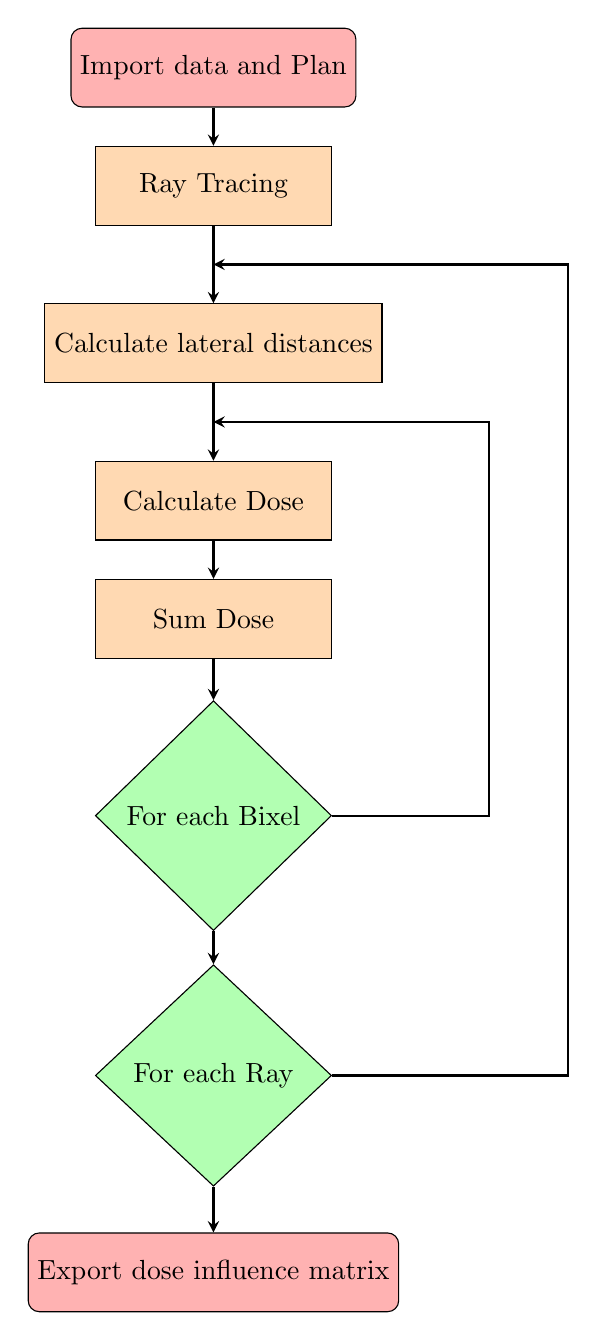
\begin{tikzpicture}[node distance=1.5cm, xshift=5cm]

\node (start) [startstop, xshift=-5cm] {Import data and Plan};

\node (rt) [process, below of=start] {Ray Tracing};
\node (geo) [process, below of=rt, yshift=-0.5cm] {Calculate lateral distances};
\node (calcdose) [process, below of=geo, yshift=-0.5cm] {Calculate Dose};
\node (store) [process, below of=calcdose] {Sum Dose};

\node (loopbixel) [decision, below of=store, yshift=-1cm] {For each Bixel};
\node (loopray) [decision, below of=loopbixel, yshift=-1.8cm] {For each Ray};

\node (end) [startstop, below of=loopray, yshift=-1cm] {Export dose influence matrix};

\node[coordinate] (r_store) [right of=store, xshift=2cm] {};
\node[coordinate] (r_loopbixel)   [right of=loopbixel, xshift=2cm] {};
\node[coordinate] (bef_dose) [below of=geo, yshift=0.5cm] {};
\node[coordinate] (r_bef_dose) [right of=bef_dose, xshift=2cm] {};
\node[coordinate] (bef_calcdose) [below of=rt, yshift=0.5cm] {};
\node[coordinate] (r_bef_calcdose) [right of=bef_calcdose, xshift=3cm] {};
\node[coordinate] (r_loopray)   [right of=loopray, xshift=3cm] {};

\node[coordinate] (r_phantom) [right of=store, xshift=5cm] {};
\node[coordinate] (l_phantom) [left of=store, xshift=-5cm] {};


\draw [arrow] (start) -- (rt);
\draw [arrow] (rt) -- (geo);
\draw [arrow] (geo) -- (calcdose);
\draw [arrow] (calcdose) -- (store);
\draw [arrow] (store) -- (loopbixel);
\draw [arrow] (loopbixel) -- (loopray);
\draw [arrow] (loopray) -- (end);

\draw[arrow] (loopbixel) -- (r_loopbixel) -- node[midway, left]{}  (r_bef_dose) -- (bef_dose) ;
\draw[arrow] (loopray) -- (r_loopray) -- node[midway, left]{}  (r_bef_calcdose) -- (bef_calcdose) ;

\end{tikzpicture}
\caption{Pencil beam algorithm flowchart. This is repeated for every direction of irradiation}
\label{tikz:pba}
\end{figure}
\newpage

\subsection{Pencil beam fine sampling}\label{FS}
A modified version of the pencil beam algorithms consists in the \emph{fine sampling}\footnote{Soukup (et al.) \cite{souk:pba}, describes the overall methods behind the fine sampling pencil beam and shows some of the results}.
The main difference is that fine sampling, as the name suggests, does not calculate the dose for the whole bixel in one step but divides the bixel in smaller sub-beams and repeats the dose calculation for all of them. 
\begin{figure}[t]
{\includegraphics[width=.5\textwidth]{Images/FurtherSigmaAnalysis2_01}}
{\includegraphics[width=.5\textwidth]{Images/FurtherSigmaAnalysis2_02}}
\caption{$\gamma$-index value (compared with MC) and maximum percentage error, variating $\sigma_{sub}$, for the inhomogeneous phantom. The red line means the gamma index value of matRad simulation.}
\label{fig:sigsub}
\end{figure}

The first part of the code is very similar. But before running the loop over the bixels, we need to assign a weight to the sub-components. These are arranged on a square grid at regular distance one from another, covering $3\,\sigma$ of the lateral spread of the beam profile. 
The gaussian profile of the beam (with standard deviation $\sigma$) and the profile given by the sum of the components (with standard deviation $\sigma_{sub}$) should be equal
\[
\frac{1}{\sqrt{2 \pi}\,\sigma}e^{(x^2+y^2)/2\sigma^2} = \sum_{i=1}^N \frac{w_i}{2 \pi\sigma_{sub}}e^{[(x-\mu_{xi})^2+(y-\mu_{yi})^2]/2\sigma_{sub}^2}
\]
Where $N$ is the number of sub-components, $\mu_{xi}$ and $\mu_{yi}$ are the grid point and $w_i$ are the weights of each component.
A component near to the center should give a higher contribution than a component further away and they do not have the same impact on the dose. So I imposed the weights to be gaussian shaped and I used a function that finds the correct weights, minimizing the square of the difference between the aforesaid functions.
In formula
\[
\sum^M_{j=1}\, \bigg|\frac{1}{2\pi\sigma}e^{(x_j^2+y_j^2)/2\sigma^2}\, - \sum^N_{i=1} \,\frac{W}{2\pi\Sigma}e^{(x_j^2+y_j^2)/2\Sigma^2} \,\frac{1}{2\pi\sigma_{sub}}e^{[(x_j-\mu_{xi})^2+(y_j-\mu_{yi})^2]/2\sigma_{sub}^2} \bigg|^2
\]
Where $M$ is the number of points on which the minimization run, $W$ and $\Sigma$ are the parameters of the minimization.
I run simulations on all the configuration, with $\sigma_{sub}/\sigma$ by varying from 0.1 to 0.8. 
The value of $\sigma_{sub}$ has been chosen on the basis of the accuracy of these simulations (evaluated with $\gamma$-index test\footnote{Discussed in detail in section \ref{sec:gam}}, compared with Monte Carlo simulations) and the maximum error (on the difference between gaussian profile and sum of gaussians).
In figure \ref{fig:sigsub}, you can see the results for one of the cases. The results are very similar for every phantom and from these we obtained that the most suitable value for our purposes is $\sigma_{sub}/\sigma=0.25$ because it has the highest gamma-index between the values with an error smaller than $1\%$.
\begin{figure}[t]
{\includegraphics[width=.5\textwidth]{Images/gaugrid_2}}
{\includegraphics[width=.5\textwidth]{Images/gausurf_plus}}
\caption{Gaussian lateral profile with highlighted position of the sub-components (left). Gaussian profile of sub-components (right)}
\label{fig:gaugrid}
\end{figure}

%%% adjust sigma figures: -xlabel;  -repeat calculations;  -

%%%% da fare:
%%%%		- ricalcolare gamma index e computation time per numero di sub-components
%%%%		- ricalcolare gamma index e max percentage error per sigma
%%%%		- aggiungere grafici ottenuti
%%%%		- infornare a 180° per un'ora

%%% add sigma further analysis

The other novelty introduced into the code is a function that projects the radiation depth on the central axis of every sub-component. In other words, a new ray tracing for the smaller sub-beams.
Then the radiation depth, used for rescaling longitudinal distances, is recalculated only for the central axis of the single sub-beam (e.g., the Bragg peak is not deformed, it is only scaled on the direction of the beam). I would like to focus the attention of the reader on this point. The sub-component does not take in account the general morphology of the target but only the one corresponding to the voxels crossed by its central axis. In other words, it does not take in account inhomogeneities near the sub-beam axis if they are not \emph{on} the axis. I will show in details this issue in the next chapter. 
In order to compensate this deficiency, a large number of sub-beams should be used. 
As can be easy to forecast, the higher is the number of sub-beams the higher is the accuracy of the simulation. 
The number of sub-components used is $N=324$. This number has been chosen after analysis on computation time, more than accuracy. As one can see from figure \ref{fig:gausn}, the gain in accuracy is almost irrelevant compared with the loss in computation time. For high $N$, the computation has also other problems, such as memory size issues because of the huge amount of data in the RAM.
\begin{figure}[t]
{\includegraphics[width=.5\textwidth]{Images/gamman}}
{\includegraphics[width=.5\textwidth]{Images/timen}}
\caption{Gamma index (left) and time consumption (right) as function of $n$. The value $n$ on the $x$-axis is related with the number of compontents as $N=(2n+2)^2$}
\label{fig:gausn}
\end{figure}

The new flowchart of the model (\ref{tikz:fs}) is very similar to the previous one but with one more loop.
Apart for the weights, there is a function that allows the projection of the radiation depth of the central axis of the component on the other points of the components.

\newpage
\begin{figure}[!ht]
\centering
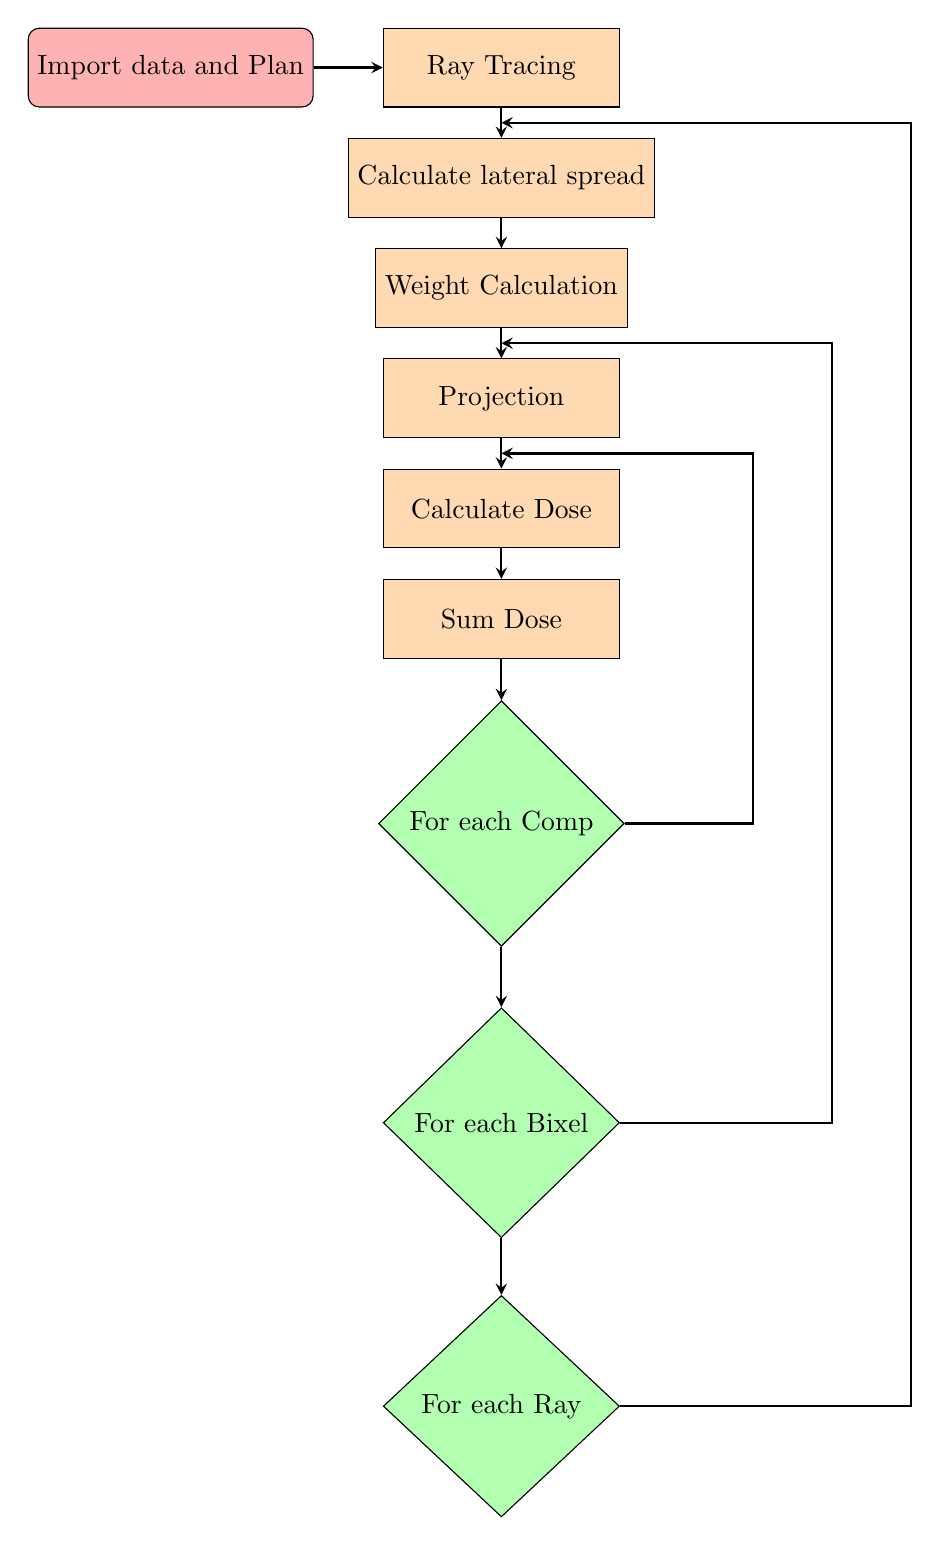
\begin{tikzpicture}[node distance=1.2cm, xshift=5cm]

\node (rt) [process] {Ray Tracing};
\node (start) [startstop, left of=rt, xshift=-3cm] {Import data and Plan};
\node (geo) [process, below of=rt, yshift=-0.2cm] {Calculate lateral spread};
\node (weight) [process, below of=geo, yshift=-0.2cm] {Weight Calculation};
\node (proj) [process, below of=weight, yshift=-0.2cm] {Projection};
\node (calcdose) [process, below of=proj, yshift=-0.2cm] {Calculate Dose};
\node (store) [process, below of=calcdose, yshift=-0.2cm] {Sum Dose};
\node (loopcomp) [decision, below of=store, yshift=-1.4cm] {For each Comp};
\node (loopbixel) [decision, below of=loopcomp, yshift=-2.6cm] {For each Bixel};
\node (loopray) [decision, below of=loopbixel, yshift=-2.4cm] {For each Ray};
%\node (end) [startstop, below of=loopray, yshift=-1cm] {Export Dose};

\node[coordinate] (r_loopcomp) [right of=loopcomp, xshift=2cm]{};
\node[coordinate] (bef_calcdose) [below of=proj, yshift=0.5cm] {};
\node[coordinate] (r_bef_calcdose) [right of=bef_calcdose, xshift=2cm] {};


\node[coordinate] (r_loopbixel)   [right of=loopbixel, xshift=3cm] {};
\node[coordinate] (bef_proj) [below of=weight, yshift=0.5cm] {};
\node[coordinate] (r_bef_proj) [right of=bef_proj, xshift=3cm] {};

\node[coordinate] (r_loopray)   [right of=loopray, xshift=4cm] {};
\node[coordinate] (bef_geo) [below of=rt, yshift=0.5cm] {};
\node[coordinate] (r_bef_geo) [right of=bef_geo, xshift=4cm] {};

\node[coordinate] (r_phantom) [right of=store, xshift=5cm] {};
\node[coordinate] (l_phantom) [left of=store, xshift=-5cm] {};


\draw [arrow] (start) -- (rt);
\draw [arrow] (rt) -- (geo);
\draw [arrow] (geo) -- (weight);
\draw [arrow] (weight) -- (proj);
\draw [arrow] (proj) -- (calcdose);
\draw [arrow] (calcdose) -- (store);
\draw [arrow] (store) -- (loopcomp);
\draw [arrow] (loopcomp) -- (loopbixel);
\draw [arrow] (loopbixel) -- (loopray);
%\draw [arrow] (loopray) -- (end);

\draw[arrow] (loopcomp) -- (r_loopcomp) -- node[midway, left]{} (r_bef_calcdose) --(bef_calcdose) ;
\draw[arrow] (loopbixel) -- (r_loopbixel) -- node[midway, left]{}  (r_bef_proj) -- (bef_proj) ;
\draw[arrow] (loopray) -- (r_loopray) -- node[midway, left]{}  (r_bef_geo) -- (bef_geo) ;
\end{tikzpicture}
\caption{Pencil beam algorithm flowchart}
\label{tikz:fs}
\end{figure}
\newpage




%b\footnote{Siemens link to Syngo page: \url{https://www.healthcare.siemens.it/medical-imaging-it}}

\section{Phantom Data}\label{phantoms}
\emph{Phantom}, in this field, is a technical word used to indicate a object built on purpose to run tests on real and physically well know devices. Building his own phantom, one can decide its physical properties in order to simplify errors detection, during numerical simulation. 

\subsection{Software Phantoms}
\label{sec:pha}
\begin{figure}[h]
{\includegraphics[width=\textwidth]{Images/phantoms2}}
\caption{From left ro right: Homogeneous; Inhomogeneous; Airbox; and Soukup phantom}
\label{fig:phantoms}
\end{figure}
When there is need to compare dose calculation softwares, the simpliest thing to do is to ``build'' a CT that represents a phantom with features decided on purpose by the programmer. This gives the chance to test this kind of softwares in situation that can highlight their weaknesses and their strengths.


For single beam comparison, I used four types of phantoms:
\begin{itemize}
\item The homogeneous waterphantom, a simple $80\times80\times80\,mm$ water box with relative stopping power (RSP) equal to 1.
\item The inhomogeneous phantom, a box of the same dimensions as the above one but divided into halves, one half contains water and the other one contains a softer material of $0.8$ RSP. The cut is parellel to the beam direction and it is right at its center.
\item The airbox phantom, a water box of the usual dimensions with a $20\times20\times20\,mm$ air box inside. The airbox was placed in different positions.
\item The Soukup phantom \footnote{This phantom was used from Soukup (et al.) in their article about pencil beam fine sampling \cite{souk:pba}}, a waterbox with two inhomogeneities of $1.5$ and $0.4$ RSP at $30\,mm$ of depth, both $20\,mm$ width.
\end{itemize}

In figure \ref{fig:phantoms} all these phantom are shown. You may notice that all the inhomogeneities are placed in order to cut the beam in halves. The beam direction is veritcal and the beam axis is at the center of the orizontal axis.


\subsection{Water Phantom}
\begin{figure}[h]
{\includegraphics[width=0.55\textwidth]{Images/PTW_31015}}
{\includegraphics[width=0.45\textwidth]{Images/PTW_31015spec}}
\caption{Single PTW-31015 ionization chamber, on the right (left picture), and precise description of its dimensions (right picture). From PTW website accessed on July 16th.}
\label{fig:31015}
\end{figure}
In this work, I compared my dataset with a set of measurements done at Heidelberg Ion-Beam Therapy Center on a phantom. The phantom used for the measurements was a plexiglass box filled with water with a detector inside. The detector is composed by 24 ionization chambers models \emph{PTW-31015}\footnote{A complete set of specifications can be found at \url{https://www.rpdinc.com/ptw-31015-003-cc-pinpoint-chamber-976.html}} produced by PTW-Freiburg\footnote{\url{http://www.ptw.de/home_start.html?&no_cache=1}}. The ionization chambers have a cylindrical shape with vented sensitive volumes of $30\,mm^3$ ($1.45\,mm$, length $5\,mm$) and $2.9\,mm$ in external diameter (figure \ref{fig:31015}).
%% The productor declares a nominal response of $800\,pC/Gy$. (\textbf{from this i should find the error on the measurement but i miss some data})
The chambers are arranged in 6 lines on 3 levels, inside a plexiglass support that allows to immerse the chambers directly into the water. In figure \ref{fig:24cham} the set up of the detector is shown.
The colleagues of the Heidelberg Ion-Beam Therapy Center collected data from measurements in nine different positions where the whole detector was moved inside the volume and across the surface of a cubic target area. More about these measurements will be reported in the next chapter.

\begin{figure}[h]
{\includegraphics[width=.5\textwidth]{Images/doublew}}
{\includegraphics[width=.5\textwidth]{Images/doublew2}}
\caption{Three-dimensional views of the \emph{Double Wedge} phantom with details of the plastic absorber (green), water (blue), target cube (red) and beam direction (black line). Scales are in tens of voxel, one voxel having a resolution of $1\times1\times1\,mm^3$}
\label{fig:doublew}
\end{figure}

\subsection{Double Wedge} 
The Double Wedges is a particular kind of phantom built by HIT colleagues with the aim of testing the effects of the treatment through a surface that has a considerable slope at the entrance surface. 
Figure \ref{fig:doublew} represents the CT of this phantom. The light blue box is the limit of the matrix and its dimensions are $512\times512\times390\,mm$. The black line is the direction of the beam and points towards $-x$ direction (or in other words, from the air side toward the water). The line passes though a point called \emph{Isocenter} and marked with a red cross. It represents the center of the axis in the machine reference system.
The actual phantom is a parallelepiped of plastic (with a known attenuation coefficient) filled with water. Its dimensions are around $500\times200\times350\,mm^3$. Along the beam direction, with comparable dimensions, there is a \emph{double wedge}, i.e., a couple of triangular plastic attenuators of $1.165$ relative stopping power. These attenuators have a gradient of $30$ and $60^\circ$, respectively.
The red square box with side of $50\,mm$ is the target where we want to release the greatest part of the dose. 

\section{Analysis techniques}
All the simulations collected during this study, should finally be compared one another. 
In fact, the key problem in this work is, to find a discriminating factor that could establish if one simulation is more or less accurate than another one. Two three-dimensional matrices can be compared in many ways, but is it possible to find a method that gives us a complete analysis and a simple way to construct it?
This is not a simple question to deal with. 

Furthermore, there is a problem in showing the result. For example, if one plots only a slide of a 3D-matrix, he could highlight some lacks and do not see others. Then we need a method that qualitatively tells us where the issue is and how much it influences the results.

In order to validate this work, I used three different kinds of comparison. In this section, I will explain them.

\subsection{Dose difference Maps}
\begin{figure}[t!]
\includegraphics[width=\textwidth]{Images/diffmap2}
\caption{Bragg peak (upper left) and dose difference maps. Axis in $cm$}
\label{fig:diff}
\end{figure}
The first and most intuitive method is to calculate the strict difference, element-by-element, between the two matrices I want to compare. Conceptually it is very simple. If we want to obtain the difference map between matrix $A$ and $B$, we define the generic element of $C$, as
\[
C_{ijk} = A_{ijk} - B_{ijk}
\]
The resulting matrix should now be plotted in a comprehensible way. In figure \ref{fig:diff}, there is a plot of a slice of a dose deposition cube (i.e., a bragg peak, in the upper left) and the difference between that cube and the same one, translated of $0.5\,mm$ towards right on the orizontal axis. 
The difference maps are plotted in different ways: the first one is a slide of the difference-dose matrix and it is plotted flat with a colormap; on the lower left, there are the same data but plotted in 3D; the last one instead is the tridimensional representation of the whole dose-difference cube, given with similar color-code.

Given the simmetry, the 3D graphs do not tell us anything new, that is why we will always show Dose difference maps using the upper-right graph.

A point to focus on is that the maximum error is over the $10\%$ of the maximum value of the dose deposition. In addition, the \emph{percentage difference}\footnote{In all this work, I will refer to percentage difference as the difference point-by-point between $A$ and $B$, divided the maximum of $A$, times 100} has an average value of $3.5\%$ (in the area where dose is above $1\%$ of the maximum). 
This seems to be a large disagreement. Instead, it is the same dose shifted only of half a millimetre, that can be considered reasonably inside our error. The result derives from the fact that we are subtracting two curves with high gradients. So, we should find a better way to account for this.

\subsection{Dose Profiles}
\label{sec:dose_prof}
To have a better prospective on the comparison between high gradient curves,
\begin{wrapfigure}{l}{.5\textwidth}
\vspace{-5mm}
{\includegraphics[width=0.5\textwidth]{Images/prof}}
\caption{Profiles example}
\label{fig:prof}
\vspace{-5mm}
\end{wrapfigure}
\noindent these should look at dose profiles. 
These are the dose values taken from a line of voxels and plotted in relation to their position. For example, if I want to see the dose profile along the center of the beam, I should select the dose value of the voxels traversed by the beam axis and plot them with their corresponding position.
In figure \ref{fig:prof}, there are shown the most common examples: \emph{i)} the entrance profile, (normally) depending only by the machine properties; \emph{ii)} the peak profile, with notable gaussian shape and \emph{iii)} the central profile, usually refered to as the \emph{Depth-Dose Profile} (DDP). There is another important DDP that is used for displaying the total dose as a function of the depth: it is called \emph{Integrated-Depth-Dose profile} (IDDP). This is similar to DDP but it takes not only a line of voxels, but a whole plane (or volume) and sums all the elements on the direction perpendicular to the beam axis, obtaining the same thing as DDP but integrated on the lateral direction.

This method represents a better way to compare two high gradient curves but it is not enough. We need a discriminator that can give us a simple and fast way to judge if a simulation is more accurate than another one.


\subsection{Gamma Index}
\label{sec:gam}
The peculiar attribute of the dose deposition simulations is to have large flat or low-gradient zones, usually inside and outside the target area (tumor in real cases) and very-high-gradient zones in the region surrounding it.
The mathematical difference between two datasets will not give us a full and exhaustive comparison because it could highlight an area of significant disagreement near high-gradient regions and a more quantitative assessment may be needed for final system approval.   
We need an instrument that could give us an estimation of accuracy in dose difference and in \emph{distance} (like the Dose profile does).
In order to get this, I used the method shown in Low (et al.) \cite{low:gamma} or else the \emph{gamma-index test} that uses a distance-to-agreement (DTA) distribution to determine the acceptability of the dose calculation. 
The distance between the two nearest voxels (of the two compared matrices) that have the same dose is called DTA. Distance and dose difference are calculated for every voxel and checked if they exceed the respective tolerance limits. Points are valued on the basis of the obtained result by appling these criteria. This method provides an index for every voxel (further called $gamma$-index) that indicates agreement (or disagreement) between regions that pass (or fail) the test.
In mathematical terms, (comparing matrix $A$ with subscript $a$ and $B$ with subscript $b$) the gamma index is
\[
\gamma(r_a) = min\{\Gamma(r_a,r_b) \}\,\,\,\,\forall\{ r_b\}
\]
where
\[
\Gamma(r_a,r_b) = \sqrt{\frac{r^2(r_a,r_b)}{\Delta d^2_M} + \frac{\delta^2(r_a,r_b)}{\Delta D^2_M}}
\]
In this formulation, $r^2(r_a,r_b)$ is the distance and $\delta^2(r_a,r_b)$ is the dose difference between two point of $A$ and $B$. Instead, $\Delta d^2_M$ and $\Delta D^2_M$ are the criteria for distance and Dose, respectively.
These criteria represent the acceptance value that we want to assign to our comparison. For example: if we have a matrix with a resolution of $3\times3\times3\,mm$, a distance criteria $\Delta d^2_M = 3\,mm$ would be the optimal one. So, if the matrix $B$ has a point with the same dose value as the point $r_a$, at a distance smaller than $3\,mm$, the gamma index test is passed for that point $r_a$.
In general, the pass-fail criteria therefore become
\[
\gamma(r_a)\leq1\,\,\,\,\,\,\textrm{calculation passes}
\]
\[
\gamma(r_a)>1\,\,\,\,\,\,\textrm{calculation fails}
\]
The output of this test is usually given in percentage of points passing the test on the total number of points of the matrix.
From this result, the points with dose value smaller than $\Delta D^2_M$ criteria are excluded.
Ad the end, we finally built the instrument that we needed. Anyway, in the next chapter I will expose the results using all the aforesaid methods.



\begin{figure}[b]
{\includegraphics[width=\textwidth]{Images/Siemens24chambers}}
\caption{Photographs of the complete mounted detector from different points of view. Provided by the technitians of Heidelberg Ion-beam Therapy Center}
\label{fig:24cham}
\end{figure}




\chapter{Results} \label{res}%%%%%%%%%%%%%%%%%%%%%%%%%%%%%%%%%%%%%%%%%%%%%%%%%%%%%%%%%%%%%%%%%
\label{chap:res}

This chapter shows the results obtained for different cases, starting from the simplest one to exploring more complicated and realistic treatment fields in order to give an accurate and full comparison between the different algorithms described in chapter \ref{MatMeth}. 

The elementary beams section describes the results for proton beams at the following energies: $125\,MeV$ for the first three phantoms; $125\,MeV$ and $172\,MeV$ for the Soukup phantom; $21\,MeV$, $125\,MeV$ and $172\,MeV$ for the double wedge phantom.

%---------------------------------------------------ELEMENTARY PENCIL BEAMS-----------------------------------
\section{Elementary pencil beams}
%\begin{figure}[h!]
%\centering
%\vspace{-10mm}
%\includegraphics[width=0.8\textwidth]{Images/images_thesis/homo_dose}
%\caption{Dose deposition in water box for (from left to right) matRad, fine sampling, Monte Carlo}
%\label{fig:WB1}
%\end{figure}

\begin{figure}[!b]
\centering
\subfloat[][\emph{matRad}]
{\includegraphics[width=.25\textwidth]{Images/Images_homo/mR_FSBvsMC_pub_homog_02}}\quad
\subfloat[][\emph{fine sampling}]
{\includegraphics[width=.25\textwidth]{Images/Images_homo/mR_FSBvsMC_pub_homog_03}}\quad
\subfloat[][\emph{Monte Carlo}]
{\includegraphics[width=.25\textwidth]{Images/Images_homo/mR_FSBvsMC_pub_homog_04}}\quad
\caption{Dose deposition in water box.}
\label{fig:WB1}
\vspace{-20mm}
\end{figure}
The main idea behind the comparison between similar simulation methods is to exhibit their similarities for the very simple cases at first. Therefore, one is allowed analyse more and more sophisticated problems. 
A typical treatment plan consists of thousands of elementary pencil beams (i.e., the ones calculated for each bixel). In a full field simulation, an hypothetical small error on the single pencil beam can be summed over all the bixels, resulting in a very significant systematic error.

%---------------------------------------------------WATER BOX-----------------------------------

\subsection{Water Box}
The easiest case is represented by a symmetric cube of water called \emph{Water Box} used as environment for the simulation. The use of the Water Box has the aim to test the method in order to show the presence of any mistakes in the code. Furthermore, this test produce a typical Bragg peak as sum of many Bragg peaks. 
The dose simulations has given us the result shown in figure \ref{fig:WB1}, where the Isocenter slice of the dose cubes is plotted.



The full agreement of these data sets can be confirmed by the percentage difference map and the $\gamma$-index test, as shown in Figure \ref{fig:WB1gam}.
\begin{figure}[!ht]
\centering
\subfloat[][\emph{Percentage\\ difference}]
{\includegraphics[width=.25\textwidth]{Images/Images_homo/mR_FSBvsMC_pub_homog_05.png}} 
\subfloat[][\emph{$\gamma$-index \\ $99.92\%$ [$1\%$ $1mm$]}]
{\includegraphics[width=.25\textwidth]{Images/Images_homo/mR_FSBvsMC_pub_homog_06.png}}
\subfloat[][\emph{Percentage\\ difference}]
{\includegraphics[width=.25\textwidth]{Images/Images_homo/mR_FSBvsMC_pub_homog_07.png}} 
\subfloat[][\emph{$\gamma$-index \\ $99.92\%$ [$1\%$ $1mm$]}]
{\includegraphics[width=.25\textwidth]{Images/Images_homo/mR_FSBvsMC_pub_homog_08.png}} 
\caption{Comparison between matRad and Monte Carlo (left), fine sampling and Monte Carlo (right) in water box.}
\label{fig:WB1gam}
\end{figure}

An important feature to observe is the light shift in the Bragg peak position. From the central profile (in figure \ref{fig:WB1prof}), we have measured a shift of $0.13\pm0.10\,mm$ and $0.12\pm0.10\,mm$ in the direction of the beam for fine sampling and matRad, respectively. In figure \ref{fig:WB1prof} is shown a zoomed image of both these profiles.
The measured integral dose is $103.3\,cGy$ for matRad, $103.0\,cGy$ for fine sampling and $103.7\pm1.0\,cGy$ for Monte Carlo simulations.\\
\\

\begin{figure}[!ht]
\centering
\subfloat[][\emph{Central Dose profile}]
{\includegraphics[width=.45\textwidth]{Images/Images_homo/mR_FSBvsMC_pub_homog_09.png}} 
\subfloat[][\emph{Integrated Depth Dose profile}]
{\includegraphics[width=.45\textwidth]{Images/Images_homo/mR_FSBvsMC_pub_homog_10.png}} \\
\subfloat[][\emph{Phantom surface entering profile}]
{\includegraphics[width=.45\textwidth]{Images/Images_homo/mR_FSBvsMC_pub_homog_11.png}} 
\subfloat[][\emph{Peak profile}]
{\includegraphics[width=.45\textwidth]{Images/Images_homo/mR_FSBvsMC_pub_homog_12.png}}
\caption{Profiles in water box simulation.}
\label{fig:WB1prof}
\end{figure}

%\begin{figure}[!ht]
%\centering
%\subfloat[][\emph{Central Dose profile}]
%{\includegraphics[width=.45\textwidth]{Images/Images_homog_phantom/CP_wb_zoom.png}} 
%\subfloat[][\emph{Integrated Depth Dose profile}]
%{\includegraphics[width=.45\textwidth]{Images/Images_homog_phantom/IDD_wb_zoom.png}}
%\caption{Profiles in water box simulation, zoomed}
%\label{fig:WB1profz}
%\end{figure}

\begin{figure}[!b]
\centering
\subfloat[][\emph{matRad}]
{\includegraphics[width=.25\textwidth]{Images/Images_homo/mR_FSBvsMC_pub_homog_15.png}}\quad
\subfloat[][\emph{fine sampling}]
{\includegraphics[width=.25\textwidth]{Images/Images_homo/mR_FSBvsMC_pub_homog_16.png}}\quad
\subfloat[][\emph{Monte Carlo}]
{\includegraphics[width=.25\textwidth]{Images/Images_homo/mR_FSBvsMC_pub_homog_17.png}}\quad
\caption{Dose deposition in water box, $30^\circ$ degree entering beam.}
\label{fig:WB2}
\end{figure}

%---------------------------------------------------30 DEGREES-----------------------------------

\subsubsection{Beam entering at $30^\circ$ degrees}\label{30degrees}

\begin{figure}[!t]
\centering
\subfloat[][\emph{Percentage\\ difference}]
{\includegraphics[width=.25\textwidth]{Images/Images_homo/mR_FSBvsMC_pub_homog_18.png}} 
\subfloat[][\emph{$\gamma$-index \\ $98.77\%$ [$1\%$ $1mm$]}]
{\includegraphics[width=.25\textwidth]{Images/Images_homo/mR_FSBvsMC_pub_homog_19.png}}
\subfloat[][\emph{Percentage\\ difference}]
{\includegraphics[width=.25\textwidth]{Images/Images_homo/mR_FSBvsMC_pub_homog_20.png}} 
\subfloat[][\emph{$\gamma$-index \\ $96.30\%$ [$1\%$ $1mm$]}]
{\includegraphics[width=.25\textwidth]{Images/Images_homo/mR_FSBvsMC_pub_homog_21.png}} 
\caption{Comparison between matRad and Monte Carlo (left), fine sampling and Monte Carlo (right) in water box.}
\label{fig:WB2gam}
\end{figure}

\begin{figure}[!b]
\centering
\subfloat[][\emph{Integrated Depth Dose profile}]
{\includegraphics[width=0.31\textwidth]{Images/Images_homo/mR_FSBvsMC_pub_homog_22.png}}\quad
\subfloat[][\emph{Central Dose profile}]
{\includegraphics[width=0.31\textwidth]{Images/Images_homo/mR_FSBvsMC_pub_homog_24.png}}\quad
\subfloat[][\emph{Peak profile}]
{\includegraphics[width=0.31\textwidth]{Images/Images_homo/mR_FSBvsMC_pub_homog_25.png}}\quad
\caption{Profiles in water box simulation.}
\label{fig:WB2prof}
\end{figure}

This paragraph describes a beam entering the phantom at an angle of $30^\circ$ degrees. This case is fundamental to understand the major differences between matRad and the fine sampling algorithm. In figure \ref{fig:WB2}, we can see that the shape of the dose depositions obtained with the two algorithms is significantly different from the one obtained in the Monte Carlo simulation. Therefore, we can infer that the Monte Carlo simulation stays in between two extremely different interpretations.
The reason they behave so differently from the Monte Carlo simulation lies in the evaluation of the radiation depth. Indeed, matRad as software based on \emph{Ray Casting} calculates the radiation depth for every possible particle direction (parallel to the main beam) and adjusts the Bragg peak pre-computed in water to the radiation depth previously calculated. Conversely, Fine sampling divides the incoming particle fluence into several sub-beams whose radiation depth is evaluated singularly and only on the central axis of the sub-sample, giving a better sensitivity to the morphology of the target but, on the other hand, a bad response to small inhomogeneities inside the tissue.
This is the reason for the considerable shift of the Bragg Peak in the central and lateral dose profile of the peak, shown in figure \ref{fig:WB2prof}. The shift has been calculated to be $0.4\pm0.3\,mm$ in the fine sampling algorithm and $0.7\pm0.4\,mm$ in the matRad algorithm. This can be considered an important result despite the $3mm$ resolution of the CT data.
The total Dose deposited is $811.9$, $810.2$ and $813.2\pm8.1\,cGy$ for matRad, fine sampling and Monte Carlo, respectively.

\begin{figure}[!h]
\centering
\subfloat[][\emph{matRad}]
{\includegraphics[width=.31\textwidth]{Images/Images_homo/mR_FSBvsMC_pub_homog_27.png}} 
\subfloat[][\emph{Fine sampling}]
{\includegraphics[width=.31\textwidth]{Images/Images_homo/mR_FSBvsMC_pub_homog_28.png}}
\subfloat[][\emph{Monte Carlo}]
{\includegraphics[width=.31\textwidth]{Images/Images_homo/mR_FSBvsMC_pub_homog_29.png}} \\
\subfloat[][\emph{Integrated Depth Dose profile}]
{\includegraphics[width=.31\textwidth]{Images/Images_homo/mR_FSBvsMC_pub_homog_35.png}}
\subfloat[][\emph{Phantom surface entering profile}]
{\includegraphics[width=.31\textwidth]{Images/Images_homo/mR_FSBvsMC_pub_homog_36.png}}
\subfloat[][\emph{Peak Profile}]
{\includegraphics[width=.31\textwidth]{Images/Images_homo/mR_FSBvsMC_pub_homog_37.png}}
\caption{Profiles in water box simulation and Profiles in water box simulation,  $45^\circ$ degree entering beam.}
\label{fig:WB3prof}
\end{figure}

%---------------------------------------------------45 DEGREES-----------------------------------

\subsubsection{Beam entering at $45^\circ$ degrees}
As third case, we have considered a beam entering at an angle of $45^\circ$ degrees. This case shows us more explicitly the issue encountered when Ray-Casting-algorithms treat surfaces with particular shapes, such as when the beam enter at the edge of the cube. In figure \ref{fig:WB3prof}, we can notice the computer-fabricated artifact in matRad simulation that reproduces the shape of the angle of the CT surface in the dose deposition. This is clearly wrong, even if the Monte Carlo simulation outlines the same behaviour in a smoother way. Fine sampling produces a wrong interpretation caused by the weights assigned to the sub-beams. In other words, it gives to the central beam almost twice the weight of the nearest lateral sub-beams and almost 20 times more compared with the sub-components at $3\sigma$.
Nevertheless, this issue does not compromise the accuracy of the fine sampling simulation, as confirmed by the comparison tests shown in figure \ref{fig:WB3gam} and figure \ref{fig:WB3prof}. From these tests, a shift of $0.3\pm0.3\,mm$ for the fine sampling and $0.9\pm0.7\,mm$ for matRad in the beam direction were measured. Additionally, we obtained an integrated Dose of $946.8$, $940.3$ and $951.5\pm10.7\,cGy$ for matRad, the fine sampling and the Monte Carlo, respectively.

\begin{figure}[!ht]
\centering
\subfloat[][\emph{Percentage\\ difference}]
{\includegraphics[width=.25\textwidth]{Images/Images_homo/mR_FSBvsMC_pub_homog_30.png}} 
\subfloat[][\emph{$\gamma$-index \\ $96.62\%$ [$1\%$ $1mm$]}]
{\includegraphics[width=.25\textwidth]{Images/Images_homo/mR_FSBvsMC_pub_homog_31.png}}
\subfloat[][\emph{Percentage\\ difference}]
{\includegraphics[width=.25\textwidth]{Images/Images_homo/mR_FSBvsMC_pub_homog_32.png}} 
\subfloat[][\emph{$\gamma$-index \\ $99.90\%$ [$1\%$ $1mm$]}]
{\includegraphics[width=.25\textwidth]{Images/Images_homo/mR_FSBvsMC_pub_homog_33.png}} 
\caption{Comparison between matRad and Monte Carlo (left), fine sampling and Monte Carlo (right) in water box.}
\label{fig:WB3gam}
\end{figure}

%---------------------------------------------------INHOMO-----------------------------------

\subsection{Inhomogeneous Water Box}\label{inhomo}

\begin{figure}[!b]
\centering
\subfloat[][\emph{matRad}]
{\includegraphics[width=0.25\textwidth]{Images/Images_inhomo/mR_FSBvsMC_pub_inhomog_02.png}}\quad
\subfloat[][\emph{fine sampling}]
{\includegraphics[width=0.25\textwidth]{Images/Images_inhomo/mR_FSBvsMC_pub_inhomog_03.png}\label{fig:IPgam_FS}}\quad
\subfloat[][\emph{Monte Carlo}]
{\includegraphics[width=0.25\textwidth]{Images/Images_inhomo/mR_FSBvsMC_pub_inhomog_04.png}}\quad
\caption{Profiles in water box simulation.}
\label{fig:IP}
\end{figure}

The inhomogeneous water box consists in a cube divided into two parts along the beam direction. One part of the cube is filled with water while the other one is filled with a material characterised by a slightly smaller stopping power, here called \emph{gum} for simplicity. The aim of this chapter is to show how Ray Casting algorithms sees this kind of phantoms.

The results for the dose calculated by Ray Casting clearly exhibit a distinct step, as shown in figure \ref{fig:IP}. The presence of this step is caused by the same mechanism as the one discussed in \ref{30degrees}, i.e., the way matRad evaluates the radiation depth. 
From the comparison between fine sampling and Monte Carlo simulation, we can observe a much greater similarity.
In the case of matRad, we have obtained $95.72\%$ of passing points with a [$3\%$ $3mm$] criterion, differing from the $97.68\%$ of the fine sampling under the same conditions. 
Then, it is clear that a disadvantage of the algorithm in this experiment consists in a resulting not-smooth dose in both sides of the phantom. However, a method can be adopted in order to solve this issue, that is the use of a fine sampling model with a great number of sub-beams so as to make them narrower and with a more balanced weight. So, I have decided to set the number of beams at 324, leading to an improvement of the accuracy above matRad's accuracy, as can be seen in the dose deposition in figure \ref{fig:IP} and from comparisons in figure \ref{fig:IPgam}.
\begin{figure}[!ht]
\centering
\subfloat[][\emph{Percentage\\ difference}]
{\includegraphics[width=.25\textwidth]{Images/Images_inhomo/mR_FSBvsMC_pub_inhomog_05.png}} 
\subfloat[][\emph{$\gamma$-index \\ $95.62\%$ [$3\%$ $3mm$]}]
{\includegraphics[width=.25\textwidth]{Images/Images_inhomo/mR_FSBvsMC_pub_inhomog_06.png}}
\subfloat[][\emph{Percentage\\ difference}]
{\includegraphics[width=.25\textwidth]{Images/Images_inhomo/mR_FSBvsMC_pub_inhomog_07.png}} 
\subfloat[][\emph{$\gamma$-index \\ $97.68\%$ [$3\%$ $3mm$]}]
{\includegraphics[width=.25\textwidth]{Images/Images_inhomo/mR_FSBvsMC_pub_inhomog_08.png}} 
\caption{Comparison between matRad and Monte Carlo (left), fine sampling and Monte Carlo (right) in water box.}
\label{fig:IPgam}
\end{figure}

\begin{figure}[]
\centering
\subfloat[][\emph{Water central profile}]
{\includegraphics[width=.45\textwidth]{Images/Images_inhomo/mR_FSBvsMC_pub_inhomog_09}\label{fig:IPprof_wcp}} 
\subfloat[][\emph{Plastic central profile}]
{\includegraphics[width=.45\textwidth]{Images/Images_inhomo/mR_FSBvsMC_pub_inhomog_10.png}\label{fig:IPprof_pcp}}\\
\subfloat[][\emph{Integrated Depth Dose profile}]
{\includegraphics[width=.45\textwidth]{Images/Images_inhomo/mR_FSBvsMC_pub_inhomog_11.png}} 
\subfloat[][\emph{Phantom surface entering profile}]
{\includegraphics[width=.45\textwidth]{Images/Images_inhomo/mR_FSBvsMC_pub_inhomog_12.png}}\\
\subfloat[][\emph{Water peak profile}]
{\includegraphics[width=.45\textwidth]{Images/Images_inhomo/mR_FSBvsMC_pub_inhomog_13.png}
\label{fig:IPprof_wpp}}
\subfloat[][\emph{Plastic peak profile}]
{\includegraphics[width=.45\textwidth]{Images/Images_inhomo/mR_FSBvsMC_pub_inhomog_14.png}
\label{fig:IPprof_ppp}}\\
\caption{Profiles in water box simulation and Profiles in water box simulation,  $45^\circ$ degree entering beam.}
\label{fig:IPprof}
\end{figure}

Furthermore, one may notice that Monte Carlo simulation shows two peaks having a not symmetric shape with respect to the vertical axis. By contrast, Fine sampling shows an almost full symmetric shape of the peaks. This phenomenon derives from the shape of the sub-components, each of which is a Bragg peak. During the calculation these sub-components do not consider if they are crossing an inhomogeneity along the lateral direction or not. 
In such cases, the sub-beams are divided into two different categories: those attenuated inside a certain material such as water; those attenuated in another material differing from the previous one.
In this way, half of the components are used to build one peak and the other half is used to build the second peak. In addition, the beams which are closer to the center have a bigger weight and hence a stronger influence on the resulting shape of the peak. We can observe this feature in the profiles\footnote{The profiles \ref{fig:IPprof_wcp} \ref{fig:IPprof_pcp} are the central dose profiles, on water side and plastic side. In particular, they are two parallel lines of voxels, at 1 voxel distance} shown in figure \ref{fig:IPprof_wcp} and \ref{fig:IPprof_pcp}. It is shown that fine sampling has a very sharp peak in both cases, while this is not true for Monte Carlo that slightly decreases. On the other hand, matRad shows a behaviour completely independent from the other ones in both the profiles.
Then, we observe in a complete agreement on the left side of the first peak but a very poor agreement on the right side as shown in the $\gamma$-index map of FS (figure \ref{fig:IPgam_FS}) and in the lower peak profile\footnote{The profiles \ref{fig:IPprof_wpp} \ref{fig:IPprof_ppp} are the peak profiles, on water side and plastic side.} (figure \ref{fig:IPprof_ppp}).

As regards the Integrated Depth Dose Profile, we can see that the curve between the two peaks has a sharp gradient change in both MR and FS. Monte Carlo, on its own, is obviously smoother and the overflow of the dose is compensated with a smaller maximum. As proof, we can observe that the total Dose is $116.2$, $116.0$ and $116.4\pm1.3\,cGy$ for matRad, fine sampling and Monte Carlo, respectively.

\newpage
%---------------------------------------------------AIRBOX-----------------------------------

\begin{figure}[!t]
\centering
\subfloat[][\emph{MatRad}]
{\includegraphics[width=.25\textwidth]{Images/mR_FSBvsMC_pub_airbox/mR_FSBvsMC_pub_airbox_14}}\quad
\subfloat[][\emph{Fine Sampling}]
{\includegraphics[width=.25\textwidth]{Images/mR_FSBvsMC_pub_airbox/mR_FSBvsMC_pub_airbox_15}}\quad
\subfloat[][\emph{Monte Carlo}]
{\includegraphics[width=.25\textwidth]{Images/mR_FSBvsMC_pub_airbox/mR_FSBvsMC_pub_airbox_16}}\quad
\caption{Dose deposition in air box (case \#2).}
\label{fig:AB2}
\end{figure}


\begin{figure}[!t]
\centering
\subfloat[][\emph{MatRad}]
{\includegraphics[width=.25\textwidth]{Images/mR_FSBvsMC_pub_airbox/mR_FSBvsMC_pub_airbox_66}}\quad
\subfloat[][\emph{Fine Sampling}]
{\includegraphics[width=.25\textwidth]{Images/mR_FSBvsMC_pub_airbox/mR_FSBvsMC_pub_airbox_67}}\quad
\subfloat[][\emph{Monte Carlo}]
{\includegraphics[width=.25\textwidth]{Images/mR_FSBvsMC_pub_airbox/mR_FSBvsMC_pub_airbox_68}}\quad
\caption{Dose deposition in air box (case \#6).}
\label{fig:AB6}
\end{figure}

\subsection{Airbox Phantom}\label{air}
As introduced in chapter \ref{phantoms}, the airbox phantom is a water phantom with a small cubic air-pocket inside. This feature has the aim to test the behaviour of the softwares in situations similar to lungs and intestine treatment. 
I have repeated the simulation six times and for six different air-pocket positions. It was placed as following:

\begin{enumerate}
\item Right on the surface
\item at $5\,mm$ from the surface, in figure \ref{fig:AB2}
\item at $15\,mm$ from the surface
\item at $25\,mm$ from the surface
\item at $35\,mm$ from the surface
\item at $45\,mm$ from the surface, in figure \ref{fig:AB6}
\end{enumerate}

% add figures

In these examples, the key issue is the deposition of the dose in air. The dose deposited in a certain volume of air is lower than the dose deposited in a similar volume of water. For this reason, the Bragg peak in air is more extended in depth and this produces a smoother and lower peak. In figure \ref{fig:AB6prof_app}, one can see that there is no peak inside the air-box for MR and MC, while FS shows a clear peak. The issue is the same as the one introduced in section \ref{inhomo}. The peak on the side without air-pocket is extended laterally because of the modified Ray Casting introduced by fine sampling considering only the radiation depth (i.e the stopping power) on the central axis of the sub-component.
matRad does not encounter this problem because of the method based on Ray Casting explained in chapter \ref{FS}. It calculates the dose deposited in air as a constant. In practice, it shifts the Bragg peak of a distance equal to the air-pocket width (particularly clear in figure \ref{fig:AB6prof_app}), still considering the divergence of the beam in air.
None of the two approaches (MR and FS) is correct, because they create artefacts that considerably change the shape of the dose deposited compared to reality.

From the lateral profiles, we can get more interesting information. The shape of the MC peaks is well interpreted by FS for the first cases, while in the last cases evolves and slowly approaches the shape of MR (especially on the side without air-pocket).

\begin{figure}[!ht]
\centering
\subfloat[][\emph{\scriptsize Central Dose profile}]
{\includegraphics[width=.32\textwidth]{Images/mR_FSBvsMC_pub_airbox/mR_FSBvsMC_pub_airbox_21}} 
\subfloat[][\emph{\scriptsize Central Dose profile}]
{\includegraphics[width=.32\textwidth]{Images/mR_FSBvsMC_pub_airbox/mR_FSBvsMC_pub_airbox_22}}
\subfloat[][\emph{\scriptsize Integrated Depth Dose profile}]
{\includegraphics[width=.32\textwidth]{Images/mR_FSBvsMC_pub_airbox/mR_FSBvsMC_pub_airbox_23}}\\ 
\subfloat[][\emph{\scriptsize Entering Dose profile}]
{\includegraphics[width=.32\textwidth]{Images/mR_FSBvsMC_pub_airbox/mR_FSBvsMC_pub_airbox_24}}
\subfloat[][\emph{\scriptsize First peak profile}]
{\includegraphics[width=.32\textwidth]{Images/mR_FSBvsMC_pub_airbox/mR_FSBvsMC_pub_airbox_25}}
\subfloat[][\emph{\scriptsize Second peak profile}]
{\includegraphics[width=.32\textwidth]{Images/mR_FSBvsMC_pub_airbox/mR_FSBvsMC_pub_airbox_26}}\\
\caption{Profiles in air box simulation (case \#2).}
\label{fig:AB2prof}
\end{figure}

\begin{figure}[!ht]
\centering
\subfloat[][\emph{\scriptsize Central Dose profile}]
{\includegraphics[width=.32\textwidth]{Images/mR_FSBvsMC_pub_airbox/mR_FSBvsMC_pub_airbox_73}\label{fig:AB6prof_app}} 
\subfloat[][\emph{\scriptsize Central Dose profile}]
{\includegraphics[width=.32\textwidth]{Images/mR_FSBvsMC_pub_airbox/mR_FSBvsMC_pub_airbox_74}}
\subfloat[][\emph{\scriptsize Integrated Depth Dose profile}]
{\includegraphics[width=.32\textwidth]{Images/mR_FSBvsMC_pub_airbox/mR_FSBvsMC_pub_airbox_75}}\\ 
\subfloat[][\emph{\scriptsize Entering Dose profile}]
{\includegraphics[width=.32\textwidth]{Images/mR_FSBvsMC_pub_airbox/mR_FSBvsMC_pub_airbox_76}}
\subfloat[][\emph{\scriptsize First peak profile}]
{\includegraphics[width=.32\textwidth]{Images/mR_FSBvsMC_pub_airbox/mR_FSBvsMC_pub_airbox_77}}
\subfloat[][\emph{\scriptsize Second peak profile}]
{\includegraphics[width=.32\textwidth]{Images/mR_FSBvsMC_pub_airbox/mR_FSBvsMC_pub_airbox_78}}\\
\caption{Profiles in air box simulation (case \#6).}
\label{fig:AB6prof}
\end{figure}

\begin{figure}[!ht]
\centering
\subfloat[][\emph{Percentage\\ difference}]
{\includegraphics[width=.25\textwidth]{Images/mR_FSBvsMC_pub_airbox/mR_FSBvsMC_pub_airbox_17}} 
\subfloat[][\emph{$\gamma$-index \\ $93.95\%$ [$3\%$ $3mm$]}]
{\includegraphics[width=.25\textwidth]{Images/mR_FSBvsMC_pub_airbox/mR_FSBvsMC_pub_airbox_18}}
\subfloat[][\emph{Percentage\\ difference}]
{\includegraphics[width=.25\textwidth]{Images/mR_FSBvsMC_pub_airbox/mR_FSBvsMC_pub_airbox_19}} 
\subfloat[][\emph{$\gamma$-index \\ $97.83\%$ [$3\%$ $3mm$]}]
{\includegraphics[width=.25\textwidth]{Images/mR_FSBvsMC_pub_airbox/mR_FSBvsMC_pub_airbox_20}} 
\caption{Comparison between Fine Sampling Beam and Monte Carlo (left), MatRad and Monte Carlo (right) in air box (case \#2).}
\label{fig:AB2gam}
\end{figure}

\begin{figure}[!ht]
\centering
\subfloat[][\emph{Percentage\\ difference}]
{\includegraphics[width=.25\textwidth]{Images/mR_FSBvsMC_pub_airbox/mR_FSBvsMC_pub_airbox_69}} 
\subfloat[][\emph{$\gamma$-index \\ $95.32\%$ [$3\%$ $3mm$]}]
{\includegraphics[width=.25\textwidth]{Images/mR_FSBvsMC_pub_airbox/mR_FSBvsMC_pub_airbox_70}}
\subfloat[][\emph{Percentage\\ difference}]
{\includegraphics[width=.25\textwidth]{Images/mR_FSBvsMC_pub_airbox/mR_FSBvsMC_pub_airbox_71}} 
\subfloat[][\emph{$\gamma$-index \\ $92.51\%$ [$3\%$ $3mm$]}]
{\includegraphics[width=.25\textwidth]{Images/mR_FSBvsMC_pub_airbox/mR_FSBvsMC_pub_airbox_72}} 
\caption{Comparison between Fine Sampling Beam and Monte Carlo (left), MatRad and Monte Carlo (right) in air box (case \#6).}
\label{fig:AB6gam}
\end{figure}
%---------------------------------------------------SOUKUP-----------------------------------
\newpage

\subsection{Soukup Phantom}
As explained in section \ref{sec:pha}, I replicated a phantom used by Soukup (et al.) in \cite{souk:pba}. 
This phantom does not differ substantially from the air-box phantom because it has a low density window that cuts the beam in half. They main difference is the presence of a high-stopping-power region that can be thought as a bone. This has the aim of checking what happens in a high-gradient region, as in the inhomogeneous phantom, but restricted to a strip of determined thickness.

The experiment was made with two different energies of the beam (figures \ref{fig:SB1} and \ref{fig:SB2}), $125\,MeV$ and $172\,MeV$. One that has the bragg peak inside the inhomogeneity and another one that crosses it and deposits the dose deeper.
Knowing the behaviour of the dose deposition in airbox phantom, we can state that the result of the $\gamma$-index value is not so remarkable as it may seem. When there is a dose peak in the inhomogeneity, then fine sampling shows its limits.
Comparing the lateral profiles in the two cases on the peaks (figures \ref{}), we can see that there are no significant differences. Instead, it is clear from depth-dose profiles that FS describes a completely different behaviour, especially in the second peak where the dose maximum is almost the half of what should be. Looking at the integrated depth-dose profile, we can observe that there are small differences between the peaks, due probably to the fact that MC dose in the knee region before the peak is basically a little higher than the dose calculated by using the other methods (as we have already seen in the waterbox case) and this phenomenon is here more evident.
\begin{figure}[!t]
\centering
\subfloat[][\emph{MatRad}]
{\includegraphics[width=.25\textwidth]{Images/mR_FSBvsMC_pub_soukup/mR_FSBvsMC_pub_soukup_01}}\quad
\subfloat[][\emph{Fine Sampling}]
{\includegraphics[width=.25\textwidth]{Images/mR_FSBvsMC_pub_soukup/mR_FSBvsMC_pub_soukup_02}}\quad
\subfloat[][\emph{Monte Carlo}]
{\includegraphics[width=.25\textwidth]{Images/mR_FSBvsMC_pub_soukup/mR_FSBvsMC_pub_soukup_03}}\quad
\caption{Dose deposition in Soukup phantom at $172\,MeV$.}
\label{fig:SB1}
\end{figure}
\begin{figure}[!t]
\centering
\subfloat[][\emph{MatRad}]
{\includegraphics[width=.25\textwidth]{Images/mR_FSBvsMC_pub_soukup/mR_FSBvsMC_pub_soukup_14}}\quad
\subfloat[][\emph{Fine Sampling}]
{\includegraphics[width=.25\textwidth]{Images/mR_FSBvsMC_pub_soukup/mR_FSBvsMC_pub_soukup_15}}\quad
\subfloat[][\emph{Monte Carlo}]
{\includegraphics[width=.25\textwidth]{Images/mR_FSBvsMC_pub_soukup/mR_FSBvsMC_pub_soukup_16}}\quad
\caption{Dose deposition in Soukup phantom at $125\,MeV$.}
\label{fig:SB2}
\end{figure}
\begin{figure}[!t]
\centering
\subfloat[][\emph{Percentage\\ difference}]
{\includegraphics[width=.24\textwidth]{Images/mR_FSBvsMC_pub_soukup/mR_FSBvsMC_pub_soukup_04}} 
\subfloat[][\emph{$\gamma$-index \\ $93.80\%$ [$3\%$ $3mm$]}]
{\includegraphics[width=.24\textwidth]{Images/mR_FSBvsMC_pub_soukup/mR_FSBvsMC_pub_soukup_05}}
\subfloat[][\emph{Percentage\\ difference}]
{\includegraphics[width=.24\textwidth]{Images/mR_FSBvsMC_pub_soukup/mR_FSBvsMC_pub_soukup_06}} 
\subfloat[][\emph{$\gamma$-index \\ $96.15\%$ [$3\%$ $3mm$]}]
{\includegraphics[width=.24\textwidth]{Images/mR_FSBvsMC_pub_soukup/mR_FSBvsMC_pub_soukup_07}} 
\caption{Comparison between Fine Sampling Beam and Monte Carlo Simulations (left), MatRad and Monte Carlo Simulations (right) in Soukup phantom at $172\,MeV$.}
\label{fig:SB1gam}
\end{figure}
\begin{figure}[!t]
\centering
\subfloat[][\emph{Percentage\\ difference}]
{\includegraphics[width=.24\textwidth]{Images/mR_FSBvsMC_pub_soukup/mR_FSBvsMC_pub_soukup_17}} 
\subfloat[][\emph{$\gamma$-index \\ $94.25\%$ [$3\%$ $3mm$]}]
{\includegraphics[width=.24\textwidth]{Images/mR_FSBvsMC_pub_soukup/mR_FSBvsMC_pub_soukup_18}}
\subfloat[][\emph{Percentage\\ difference}]
{\includegraphics[width=.24\textwidth]{Images/mR_FSBvsMC_pub_soukup/mR_FSBvsMC_pub_soukup_19}} 
\subfloat[][\emph{$\gamma$-index \\ $83.77\%$ [$3\%$ $3mm$]}]
{\includegraphics[width=.24\textwidth]{Images/mR_FSBvsMC_pub_soukup/mR_FSBvsMC_pub_soukup_20}} 
\caption{Comparison between Fine Sampling Beam and Monte Carlo Simulations (left), MatRad and Monte Carlo Simulations (right) in Soukup phantom at $125\,MeV$.}
\label{fig:SB2gam}
\end{figure}
\begin{figure}[!t]
\centering
\subfloat[][\emph{\scriptsize Central Dose profile}]
{\includegraphics[width=.32\textwidth]{Images/mR_FSBvsMC_pub_soukup/mR_FSBvsMC_pub_soukup_08}} 
\subfloat[][\emph{\scriptsize Central Dose profile}]
{\includegraphics[width=.32\textwidth]{Images/mR_FSBvsMC_pub_soukup/mR_FSBvsMC_pub_soukup_09}}
\subfloat[][\emph{\scriptsize Integrated Depth Dose profile}]
{\includegraphics[width=.32\textwidth]{Images/mR_FSBvsMC_pub_soukup/mR_FSBvsMC_pub_soukup_10}}\\ 
\subfloat[][\emph{\scriptsize Entering Dose profile}]
{\includegraphics[width=.32\textwidth]{Images/mR_FSBvsMC_pub_soukup/mR_FSBvsMC_pub_soukup_11}}
\subfloat[][\emph{\scriptsize Peak profile}]
{\includegraphics[width=.32\textwidth]{Images/mR_FSBvsMC_pub_soukup/mR_FSBvsMC_pub_soukup_12}}
\subfloat[][\emph{\scriptsize Peak profile}]
{\includegraphics[width=.32\textwidth]{Images/mR_FSBvsMC_pub_soukup/mR_FSBvsMC_pub_soukup_13}}\\
\caption{Profiles in Soukup phantom simulation at $172\,MeV$.}
\label{fig:SB1prof}
\end{figure}
\begin{figure}[!t]
\centering
\subfloat[][\emph{\scriptsize Central Dose profile}]
{\includegraphics[width=.32\textwidth]{Images/mR_FSBvsMC_pub_soukup/mR_FSBvsMC_pub_soukup_21}} 
\subfloat[][\emph{\scriptsize Central Dose profile}]
{\includegraphics[width=.32\textwidth]{Images/mR_FSBvsMC_pub_soukup/mR_FSBvsMC_pub_soukup_22}}
\subfloat[][\emph{\scriptsize Integrated Depth Dose profile}]
{\includegraphics[width=.32\textwidth]{Images/mR_FSBvsMC_pub_soukup/mR_FSBvsMC_pub_soukup_23}}\\ 
\subfloat[][\emph{\scriptsize Entering Dose profile}]
{\includegraphics[width=.32\textwidth]{Images/mR_FSBvsMC_pub_soukup/mR_FSBvsMC_pub_soukup_24}}
\subfloat[][\emph{\scriptsize Peak profile}]
{\includegraphics[width=.32\textwidth]{Images/mR_FSBvsMC_pub_soukup/mR_FSBvsMC_pub_soukup_25}}
\subfloat[][\emph{\scriptsize Peak profile}]
{\includegraphics[width=.32\textwidth]{Images/mR_FSBvsMC_pub_soukup/mR_FSBvsMC_pub_soukup_26}}\\
\caption{Profiles in Soukup phantom simulation at $125\,MeV$.}
\label{fig:SB2prof}
\end{figure}

%---------------------------------------------------DOUBLE WEDGE-----------------------------------

\newpage
\subsection{Double wedge phantom}
\begin{figure}[!t]
\centering
\subfloat[][\emph{matRad}]
{\includegraphics[width=.55\textwidth]{Images/mR_FSBvsMC_pub_doublew_single/mR_FSBvsMC_pub_doublew_single_01}}\\ 
\subfloat[][\emph{fine sampling}]
{\includegraphics[width=.55\textwidth]{Images/mR_FSBvsMC_pub_doublew_single/mR_FSBvsMC_pub_doublew_single_02}}\\
\subfloat[][\emph{Monte Carlo}]
{\includegraphics[width=.55\textwidth]{Images/mR_FSBvsMC_pub_doublew_single/mR_FSBvsMC_pub_doublew_single_03}}\\
\caption{Dose deposition of a beam at an energy of $125\,MeV$ in double wedge phantom.}
\label{fig:DW1}
\end{figure}

The last single beam test was done on the double wedge phantom. From some aspects, it looks like the $45^\circ$ case in the water box, but inverted inside out. As in that case, the dose calculated by matRad is clearly artificial and unnatural. The shape of the Bragg peak calculated with fine sampling, is instead very accurate, reaching the $100\%$ agreement in the gamma index pass rate, in both cases. 
This tells us that in the double wedge phantom, the central components are more relevant than the others.
In this case, I decided to show three longitudinal profiles: the central one, where there is a good agreement between Monte Carlo and fine sampling; and two shifted of three voxel in opposite lateral directions, where there is a difference in dose in the plateau, in the initial part of the path (clearer in the most energetic beam in figures \ref{} and \ref{}).
The integrated depth-dose profile presents a poor accuracy from matRad. Given its shape, the peak of dose is distributed in backward direction and so we have that strange behavior at the maximum. Fine sampling is in line with the expectations. 
\begin{figure}[!t]
\centering
\subfloat[][\emph{matRad}]
{\includegraphics[width=.55\textwidth]{Images/mR_FSBvsMC_pub_doublew_single/mR_FSBvsMC_pub_doublew_single_17}}\\ 
\subfloat[][\emph{fine sampling}]
{\includegraphics[width=.55\textwidth]{Images/mR_FSBvsMC_pub_doublew_single/mR_FSBvsMC_pub_doublew_single_18}}\\
\subfloat[][\emph{Monte Carlo}]
{\includegraphics[width=.55\textwidth]{Images/mR_FSBvsMC_pub_doublew_single/mR_FSBvsMC_pub_doublew_single_19}}\\
\caption{Dose deposition of a beam at an energy of $172\,MeV$ in double wedge phantom.}
\label{fig:DW2}
\end{figure}
Beacuse of the shape of the phantom, I decided to show two types of lateral profile: the one used in the other cases, explained in section \ref{sec:dose_prof}; and a profile that follows the lines of the surface of the phantom, so that takes the first voxels crossed by the beam. The same thing was transposed on the peak obtaining the figures \ref{} and \ref{}.
Particular attention has to be paid to the profiles of the peaks (figure \ref{} and \ref{}). It shows the weakenesses of matRad but also the ridity of fine sampling. Because of the shape of the phantom, the natural behaviour of the beam should be to become tighter but, in both cases, the profile of fine sampling is a little wider than what should be. This is always caused by the fact that fine sampling central components account more than laterals and the largest part of the peak is composed by the central beam.

\begin{figure}[!ht]
\centering
\subfloat[][\emph{Percentage\\ difference}]
{\includegraphics[width=.43\textwidth]{Images/mR_FSBvsMC_pub_doublew_single/mR_FSBvsMC_pub_doublew_single_04}} 
\subfloat[][\emph{$\gamma$-index \\ $96.06\%$ [$3\%$ $3mm$]}]
{\includegraphics[width=.43\textwidth]{Images/mR_FSBvsMC_pub_doublew_single/mR_FSBvsMC_pub_doublew_single_05}}\\
\subfloat[][\emph{Percentage\\ difference}]
{\includegraphics[width=.43\textwidth]{Images/mR_FSBvsMC_pub_doublew_single/mR_FSBvsMC_pub_doublew_single_06}} 
\subfloat[][\emph{$\gamma$-index \\ $100\%$ [$3\%$ $3mm$]}]
{\includegraphics[width=.43\textwidth]{Images/mR_FSBvsMC_pub_doublew_single/mR_FSBvsMC_pub_doublew_single_07}} 
\caption{Comparison between fine sampling beam and Monte Carlo Simulations (down), matRad and Monte Carlo Simulations (up) for a beam at $125\,MeV$ in double wedge phantom.}
\label{fig:DW1gam}
\end{figure}

\begin{figure}[!h]
\centering
\subfloat[][\emph{Percentage\\ difference}]
{\includegraphics[width=.43\textwidth]{Images/mR_FSBvsMC_pub_doublew_single/mR_FSBvsMC_pub_doublew_single_20}} 
\subfloat[][\emph{$\gamma$-index \\ $95.35\%$ [$3\%$ $3mm$]}]
{\includegraphics[width=.43\textwidth]{Images/mR_FSBvsMC_pub_doublew_single/mR_FSBvsMC_pub_doublew_single_21}}\\
\subfloat[][\emph{Percentage\\ difference}]
{\includegraphics[width=.43\textwidth]{Images/mR_FSBvsMC_pub_doublew_single/mR_FSBvsMC_pub_doublew_single_22}} 
\subfloat[][\emph{$\gamma$-index \\ $100\%$ [$3\%$ $3mm$]}]
{\includegraphics[width=.43\textwidth]{Images/mR_FSBvsMC_pub_doublew_single/mR_FSBvsMC_pub_doublew_single_23}} 
\caption{Comparison between fine sampling beam and Monte Carlo Simulations (down), matRad and Monte Carlo Simulations (up) for a beam at $172\,MeV$ in double wedge phantom.}
\label{fig:DW2gam}
\end{figure}

\begin{figure}[!h]
\centering
\subfloat[][\emph{\scriptsize Central Dose profile}]
{\includegraphics[width=.40\textwidth]{Images/mR_FSBvsMC_pub_doublew_single/mR_FSBvsMC_pub_doublew_single_08}} 
\subfloat[][\emph{\scriptsize Central Dose profile}]
{\includegraphics[width=.40\textwidth]{Images/mR_FSBvsMC_pub_doublew_single/mR_FSBvsMC_pub_doublew_single_09}}\\
\subfloat[][\emph{\scriptsize Central Dose profile}]
{\includegraphics[width=.40\textwidth]{Images/mR_FSBvsMC_pub_doublew_single/mR_FSBvsMC_pub_doublew_single_10}}
\subfloat[][\emph{\scriptsize Integrated Depth Dose profile}]
{\includegraphics[width=.40\textwidth]{Images/mR_FSBvsMC_pub_doublew_single/mR_FSBvsMC_pub_doublew_single_11}}\\
\subfloat[][\emph{\scriptsize Entering profile}]
{\includegraphics[width=.40\textwidth]{Images/mR_FSBvsMC_pub_doublew_single/mR_FSBvsMC_pub_doublew_single_12}}
\subfloat[][\emph{\scriptsize Peak profile}]
{\includegraphics[width=.40\textwidth]{Images/mR_FSBvsMC_pub_doublew_single/mR_FSBvsMC_pub_doublew_single_13}}\\
\subfloat[][\emph{\scriptsize Surface entering profile}]
{\includegraphics[width=.40\textwidth]{Images/mR_FSBvsMC_pub_doublew_single/mR_FSBvsMC_pub_doublew_single_14}}
\subfloat[][\emph{\scriptsize Surface peak profile}]
{\includegraphics[width=.40\textwidth]{Images/mR_FSBvsMC_pub_doublew_single/mR_FSBvsMC_pub_doublew_single_15}}\\
\caption{Profiles in double wedge phantom simulation for a beam at $125\,MeV$.}
\label{fig:DW1prof}
\end{figure}

\begin{figure}[!ht]
\centering
\subfloat[][\emph{\scriptsize Central Dose profile}]
{\includegraphics[width=.42\textwidth]{Images/mR_FSBvsMC_pub_doublew_single/mR_FSBvsMC_pub_doublew_single_24}} 
\subfloat[][\emph{\scriptsize Central Dose profile}]
{\includegraphics[width=.42\textwidth]{Images/mR_FSBvsMC_pub_doublew_single/mR_FSBvsMC_pub_doublew_single_25}}\\
\subfloat[][\emph{\scriptsize Central Dose profile}]
{\includegraphics[width=.42\textwidth]{Images/mR_FSBvsMC_pub_doublew_single/mR_FSBvsMC_pub_doublew_single_26}}
\subfloat[][\emph{\scriptsize Integrated Depth Dose profile}]
{\includegraphics[width=.42\textwidth]{Images/mR_FSBvsMC_pub_doublew_single/mR_FSBvsMC_pub_doublew_single_27}}\\
\subfloat[][\emph{\scriptsize Entering profile}]
{\includegraphics[width=.42\textwidth]{Images/mR_FSBvsMC_pub_doublew_single/mR_FSBvsMC_pub_doublew_single_28}}
\subfloat[][\emph{\scriptsize Peak profile}]
{\includegraphics[width=.42\textwidth]{Images/mR_FSBvsMC_pub_doublew_single/mR_FSBvsMC_pub_doublew_single_29}}\\
\subfloat[][\emph{\scriptsize Surface entering profile}]
{\includegraphics[width=.42\textwidth]{Images/mR_FSBvsMC_pub_doublew_single/mR_FSBvsMC_pub_doublew_single_30}}
\subfloat[][\emph{\scriptsize Surface peak profile}]
{\includegraphics[width=.42\textwidth]{Images/mR_FSBvsMC_pub_doublew_single/mR_FSBvsMC_pub_doublew_single_31}}\\
\caption{Profiles in double wedge phantom simulation for a beam at $172\,MeV$.}
\label{fig:DW2prof}
\end{figure}





\newpage
\section{Realistic Treatment Fields}
\subsection{Double Wedge}
This section exposes the predictions made with matRad and Syngo and shows the comparison between them by using the $\gamma$-index test. The figures \ref{fig:SyngoMat} shown below are slices of a sagittal plane of the phantom passing through the isocenter of the CT-cube.
\begin{figure}[!ht]
\centering
\subfloat[][\emph{Syngo}]
{\includegraphics[width=.45\textwidth]{Images/Images/epub_comparison2_01.png}} \quad
\subfloat[][\emph{matRad}]
{\includegraphics[width=.45\textwidth]{Images/Images/epub_comparison2_02.png}} \quad
\caption{Simulated Double Wedges Dose deposition}
\label{fig:SyngoMat}
\end{figure}

a

\begin{figure}[t]
\centering
\subfloat[][\emph{Percentage Dose Difference}]
{\includegraphics[width=.65\textwidth]{Images/Images/epub_comparison2_03.png}} \\
\subfloat[][\emph{Gamma index test with parameters 1\% - 1$mm$}]
{\includegraphics[width=.65\textwidth]{Images/Images/epub_comparison2_04.png}} \\
\subfloat[][\emph{Gamma index test with parameters 2\% - 2$mm$}]
{\includegraphics[width=.65\textwidth]{Images/Images/epub_comparison2_05.png}} \quad
\caption{Comparison between matRad and Syngo}
\label{fig:SyngoMat2}
\end{figure}

\subsubsection{Measurements}
The last step of this thesis is to check the compatibility of our prediction with the real measurements. These are our gold standard and this is the final test that every software has to overcome to be consider a good predictor.

As said in Chapter 2, the detector inside Double Wedges Phantom has been placed in 9 different positions and, for each of them, I have the dose value measured in every chamber and that one predicted by Syngo. In this case, the simulation with Syngo has been made in two different ways. The first simulates the whole proton beam and the dose deposition inside the CT-cube (it works in the same way as matRad does), then from this cube the values of dose in the areas covered by every single chamber are extracted. The second one, referred as Syngo, evaluates the dose directly inside the area covered by every single ionization chamber; this causes a slightly difference between them.

In the following pages, I will show a series of images where there are shown a slice of the dose cube evaluated with matRad and the projection of the position of the 24 chambers, all in CT resolution. Associated to this set of images, there is a graph that reports the actual value in $cGy$ of the ionization chambers for measurements and simulations.
\newpage
\begin{figure}[h!]
\centering
\subfloat[][\emph{Sagittal plane}]
{\includegraphics[width=.65\textwidth]{Images/Images/Meas_MR_comparison_01.png}} \quad
\subfloat[][\emph{Coronal plane}]
{\includegraphics[width=.65\textwidth]{Images/Images/Meas_MR_comparison_02.png}} \\
\subfloat[][\emph{Ionization chambers values}]
{\includegraphics[width=.65\textwidth]{Images/Images/Meas_MR_comparison_03.png}} \quad
\caption{Results, geometry and comparison from configuration 1}
\label{fig:pos1}
\end{figure}

\newpage
\begin{figure}[h!]
\centering
\subfloat[][\emph{Sagittal plane}]
{\includegraphics[width=.45\textwidth]{Images/Images/Meas_MR_comparison_01.png}} \quad
\subfloat[][\emph{Coronal plane}]
{\includegraphics[width=.45\textwidth]{Images/Images/Meas_MR_comparison_02.png}} \\
\subfloat[][\emph{Ionization chambers values}]
{\includegraphics[width=.45\textwidth]{Images/Images/Meas_MR_comparison_03.png}} \quad
\caption{Results, geometry and comparison from configuration 2}
\label{fig:pos2}
\end{figure}


\chapter{Discussion} %%%%%%%%%%%%%%%%%%%%%%%%%%%%%%%%%%%%%%%%%%%%%%%%%%%%%%%%%%%%%%

\section{Summary}
In chapter \ref{res}, we have made some comparisons between simulations run by using pencil beam and fine sampling algorithms for different cases of single bixel and full field simulation, as well as Monte Carlo methods and measurements obtained at Heidelberg Ion-Therapy center.
\begin{table}[b]
\centering
\begin{tabular}{ccccc}
\toprule
Case & \multicolumn{2}{c}{matRad} & \multicolumn{2}{c}{fine sampling}\\
\midrule
 & $\gamma$-index pass rate & max $\%$ diff & $\gamma$-index pass rate & max $\%$ diff\\
\midrule
$0^\circ$ & $99.92\%$ & 1 & $99.92\%$ &1\\
$30^\circ$ & $98.77\%$ & 1 & $96.30\%$ &1\\
$45^\circ$ & $96.62\%$ & 1 & $99.91\%$ &1\\
\bottomrule
\end{tabular}
\label{tab:hom}
\caption{Results for waterbox phatom analysis}
\end{table}

We have shown the results for four different types of phantoms irradiated with a single proton beam at fixed energy.
In the case of the waterbox phantom, we have proved that there is a very good agreement between matRad, fine sampling and Monte Carlo for a beam entering at $0^\circ$ degree. The gamma-index test is over $99.9\%$ and the maximum percentage difference is less than $5\%$ for both the methods used. This result is due to a light shift in the depth.
The Bragg peaks obtained are not identical for the different algorithms because the look-up tables of matRad and, consequently, of fine sampling are obtained by using a Monte Carlo based software that works in a slightly different way compared to FLUKA.
In the other waterbox cases, we have seen that matRad is still robust in calculating the dose deposited by a beam entering at an angle of $30^\circ$ degrees on a flat surface, while it has failed the test for an  of $45^\circ$ degrees because the beam is centred on the corner of the cube, and as result, the peak is shaped in the same way. This is the main issue of ray-casting-based methods. Instead, fine sampling has shown a good approximation in the $45^\circ$ degrees case because it overcomes the problem of the corner, but it has given poorer results in the other case because of the fact that the weights are higher on the central sub-beams than on the lateral ones. In table \ref{tab:hom}, a general overview of this case is reported.

In the case of homogeneous phantom, we have seen how the three methods behave in the cases where the beam encounters a steep lateral gradient (in stopping power) on its path. The dose calculated with matlab appears sharply cut into two parts and there is no smooth transition between them. Then, it becomes evident that they look like two completely independent halves of a Bragg peak.
By contrast, Fine sampling has proved to be affected by the opposite problem. Indeed, a possible transition through a lateral gradient is not taken into account. Therefore, the Bragg peaks generated by the sub-beams cross the plane between the two materials without being affected, reflecting this on the result that shows two peaks across the inhomogeneity that are wider than expected. Concerning the gamma-index test, fine sampling has obtained a slightly better result than matRad, giving a gamma index of $97.68\%$ against the $95.62\%$ found with matRad.

\begin{figure}[!t]
\centering
{\includegraphics[width=.83\textwidth]{Images/gammacase}} 
\caption{Gamma index in relation to the case number, for FS and MR related to tab \ref{tab:air}}
\label{fig:gamcase}
\end{figure}

In the airbox case, we have proved what Schaffner (et al.) (\cite{schaf:pba}) infer on their paper. The fine sampling method is not able to describe correctly the dose deposition when the Bragg peak (or part of it) is in an area characterised by a high gradient in the CT. Starting from the fifth case, the Bragg peak is on the air-pocket and some issues occur. The gamma-index pass rate of fine sampling decreases under the value of that one we have obtained with matRad. It corresponds to the situation in which the first Bragg peak is exactly on the air-pocket. As we can see in figure \ref{fig:gamcase} and in table \ref{tab:air}, the $\gamma$-index pass rate of FS simulation decreases with the distance of the air-pocket from the surface. Conversely, matRad has shown its best agreement when fine sampling has started to fail. As explained in chapter \ref{air}, the reason lies in the dose deposited in air, which is smaller than the dose inside the tissue. This results in sharply separated beams which are more similar to the matRad's ones. We have found many analogies between the airbox and the Soukup phantom. But again, we have seen the problems of fine sampling in calculating the Bragg peak on a high gradient area. In fact, on the same phantom, it scores a gamma-index pass rate of $96.15\%$ in the case of the most energetic beam, against the $83.77\%$ of the other case where part of one peak is the high gradient area of the phantom. In such cases, the problem is not the air by itself, but the principle is the same.
As we have described, the inhomogeneity is divided into two parts. The particles that cross the edge from the higher to the smaller stopping power part have still enough energy to fly deeper into the tissue. Then, there is only half of a Bragg peak appearing in the high stopping power region that does not have a corresponding one on the other side.

\begin{table}[t]
\centering
\begin{tabular}{ccccc}
\toprule
Case & \multicolumn{2}{c}{matRad} & \multicolumn{2}{c}{fine sampling}\\
\midrule
 & $\gamma$-index pass rate & max $\%$ diff & $\gamma$-index pass rate & max $\%$ diff\\
\midrule
1 & $93.45\%$ & 1 & $98.30\%$ &1\\
2 & $98.77\%$ & 1 & $96.30\%$ &1\\
3 & $96.62\%$ & 1 & $99.91\%$ &1\\
4 & $96.62\%$ & 1 & $99.91\%$ &1\\
5 & $96.62\%$ & 1 & $99.91\%$ &1\\
6 & $96.62\%$ & 1 & $99.91\%$ &1\\
\bottomrule
\end{tabular}
\label{tab:air}
\caption{Results for airbox phatom analysis}
\end{table}

Double wedge is the example that gave us the best results, with $100\%$ agreement with Monte Carlo. Unfortunately it is just a lucky case. The outcome is so accurate because of the favourable geometry of the case. 


\section{Interpretation}
What we globally see from the results discussed in chapter \ref{res} is that matRad and fine sampling behave in complete opposite ways. Because of their intrinsic properties, Pencil beam algorithms calculate the dose deposition considering the longitudinal variation of the stopping power of the medium, i.e., on the direction of the beam only. The strength of this method is that pencil beam is robust in the other areas of the dose deposition, even if it can overestimate the correct amount of dose in the region of the Bragg peak. On the other hand, its weakness is the sharpness of the distributed dose. In the case of a considerable inhomogeneity, such as bone or air, the resulting dose is distinctly cut in different parts with no smooth transition between them. Similar is the case for a beam entering a surface characterised by a particular shape, such as the $45^\circ$ degrees waterbox case and the double wedge case, where the Bragg peak is strictly conditioned to assume an evident unnatural shape.
For its part, fine sampling tries to solve this issue so as to obtain a smoother dose. This leads to a dose deposition that does not account much on the lateral gradient in the stopping power, especially around the peak.
In conclusion, fine sampling can be very accurate in cases where the inhomogeneity is near the surface of the patient, while it is less accurate in the case of a dose deposition in areas with steep longitudinal gradients in stopping power (e.g., one of the cases of the Soukup phantom)\footnote{The clearest example is the $\gamma$-index pass rate as function of the airbox distance from the surface (figure \ref{fig:gamcase})}. Nevertheless, cases with significant inhomogeneities inside the target area (the tumor), are very rare. In fact, in the majority of the cases the target volume is homogeneous in density and it is more likely to find inhomogeneities only next to the tumor, such as in case of treatments to the basement of the head, the spine, the pelvis, the lungs, etc. In my opinion, in this cases, pencil beam would be more reliable in terms of the dose deposition in the surrounding tissues, while fine sampling would give a more accurate distribution of the dose inside the target.

About the physical shape of the peak, we can assert that none of the two methods have yielded substantial results. For the reasons explained before, pencil beam has been proven to depend too much on the shape of the phantom, sometimes being a bit contrived. Moreover, fine sampling takes into account too much on the path of the central sub-beams, that means it cares less about the inhomogeneities nearby the trajectory and that the Bragg peak is stiff under spatial deformation, just as if it always tries to keep its natural shape.

Pencil beam and pencil beam fine sampling are two methods with significant differences, with opposite strengths but almost equivalent in accuracy. We can state that \emph{in medio stat virtus}.


\section{Other Published Data}

The authors of previous studies, such as Schaffner et al. \cite{schaf:pba} and Soukup et al. \cite{souk:pba}, have been dealing with problems very similar to the ones examined in this thesis.\\
In order to solve them, Schaffner et al. \cite{schaf:pba} have proposed two methods: the Modified Ray Casting Model (MRCM), very similar to pencil beam but that takes into account also protons with lines of flight not parallel to the main beam; the Fluence-Dose Model (FDM), based on the convolution between the fluence and a kernel obtained from the look-up tables.\\
Schnider (et al.) \cite{schn:pba} have extensively described the MRCM. First, it divides every bixel in sub-components that have different entrance angles with respect to the direction of the beam. Second, it calculates the dose for each component and as last, it weights their contribution proportionally to the entrance angle. Schaffner (et al.) say about their work: \emph{They showed a good coincidence between the range spectra obtained from their analytical calculation and the Monte Carlo simulation}.\\
The second method, i.e., the FDM, proceeds in a different way. First, it uses a set of sub-beams and calculates the dose for each one. At the end, it calculates a weighted mean to obtain the total dose. In practice, this method does the same things as fine sampling but in a different order and by using the convolution.\\
In order to test these methods, they have used a phantom very similar to the airbox phantom, but with the presence of an obstacle whose stopping power is larger than water, such as a slab. As expected, these two methods have behaved very similarly to matRad and fine sampling. They have obtained (figure \ref{fig:schaff}) that the accuracy of the fluence-dose model decreases as the slab is closer to the Bragg peak. By contrast, the MRCM have shown that the agreement with MC is better when the Bragg peak cross the slab. This result is consistent with what we have seen in the aribox case.\\

%\begin{figure}[!t]
%\centering
%{\includegraphics[width=\textwidth]{Images/schaff}} 
%\caption{Example of dose percentage difference map comparison between Monte Carlo (MC), Fluence-Dose Model (FDM) and Modified Ray Casting Model (MRCM). Gray scale goes from $-10\%$ (white) to $10\%$(black). %From Schaffner (et al.) \cite{schaf:pba}.}
%\label{fig:schaff}
%\end{figure}

Soukup (et al.) \cite{souk:pba} have proposed a different solution. It consists in a version of pencil beam fine sampling based on analytical methods and not on look-up tables. The key point in this solution is the choice of the width, the number and the position of the sub-components. They have divided the beam by using only an odd number of sub-components as $N=(2n+1)^2$, while we have used an even number of sub-components as $N=(2n+2)^2$, where $n$ is an integer. Then, the method by Soukup (et al.) has a central sub-component. Conversely, we have built a method with no central sub-component in order to be more robust on central longitudinal inhomogeneities. Furthermore, the sigma of the sub-components (that we have called $\sigma_{sub}$) has been set constant as in our method, with the difference that they have imposed $\sigma_{sub}$ to be always smaller than the size of the voxel, calling this method \emph{adaptive} fine sampling. This means that if the beam has a sigma of $3\,mm$ on both axis and the voxel size is $1\,mm$, they will need at least 361 sub-beams to cover $3\sigma$. Soukup et al. have shown that if the number of sub-spots increases, then the shape description improves, but they have given no description of how this sub-components were weighted.
Some results from this authors are shown in figure \ref{fig:souk_graph}. Our results given for the same phantom are shown in figure \ref{fig:souk_fs}.

%\begin{figure}[!t]
%\centering
%{\includegraphics[width=.3\textwidth]{Images/souk_centr}} 
%{\includegraphics[width=.3\textwidth]{Images/souk_int}} 
%{\includegraphics[width=.3\textwidth]{Images/souk_prof}} 
%\caption{Dose distributions for $172\,MeV$ protons in a Soukup phantom. On the left
%side is the central axis depth dose per primary proton (mean dose of four voxels around the centre), in the middle is the integrated depth dose per primary proton and on the right side is the lateral dose profile in the depth of the first Bragg peak. Calculated with fine sampling.}
%\label{fig:souk_fs}
%\end{figure}

Soukup (et al.) have obtained a very good outcome by using the adaptive fine sampling. In the integrated depth-dose profile, we have obtained results comparable to their adaptive fine sampling. However, in other cases my method is more similar to the case (B) with 49 sub-spots. The profile plot of the adaptive fine sampling shows that they have reached great results, while fine sampling has been proved to have little agreement on this. As we can notice, the shape of the profile is different for the Monte Carlo simulations as well. Their profiles seem to be surprisingly symmetric, that could mean that they have chosen materials whose stopping powers differ from each other by a small amount. 

%\begin{figure}[!t]
%\centering
%{\includegraphics[width=\textwidth]{Images/souk_graph}} 
%\caption{Dose distributions for $100\,MeV$, $150\,MeV$ and $200\,MeV$ protons in a Soukup phantom. On the left
%side is the central axis depth dose per primary proton (mean dose of four voxels around the centre), in the middle is the integrated depth dose per primary proton and on the right side is the lateral dose profile in the depth of the first Bragg peak. (A) dose distribution with precision 0, (one sub-spot per original spot), (B) dose distribution with precision 3 (49 sub-spots) and (C) dose distribution with adaptive precision. From Soukup (et al.) \cite{souk:pba}.}
%\label{fig:souk_graph}
%\end{figure}

%Soukup (et al.) have shown a great agreement between the data and Monte Carlo. Our method is not as accurate as their but our results are coherent with all the articles.
In the end, we can assert that the method I implemented is coherent with these articles.


%------------------------------------------------------------------------------------------------------------------------------------------------------------------------------------------------------------------------
\chapter{Conclusions} %%%%%%%%%%%%%%%%%%%%%%%%%%%%%%%%%%%%%%%%%%%%%%%%%%%%%%%%%%%%%
This thesis has shown an overview of the pencil beam fine sampling. In particular, we have seen some examples of basic environments and their comparison with some existing methods. 

Fine sampling has not been treated in this thesis as an algorithm for the purposes of substituting the generic pencil beam. It could become a fast and reliable software for approximate dose calculation only by doing important modifications and the implementation of some changes in the algorithm.

In almost all the examples analysed in this thesis, we have seen that fine sampling has obtained slightly better results with respect to the pencil beam. Because of the physical approach used and the limited variety of examples discussed, I am not allowed to say that it can be considered more accurate than pencil beam. In order to improve the accuracy, one could either increase the number of sub-components or find better parameters for the sub-beams. However, this solution will not give extraordinary results.

In my opinion, there is an intrinsic limit in this method that might not be overcame. Thus, we need to change the algorithm and mix fine sampling with other methods considering the gradient of the stopping power on the plane perpendicular to the direction of the particle. For example, It could be interesting to try a convolutional smoothing method, that uses convolutional masks in order to smooth the dose and obtain an effect of lateral spreading.

Concerning the time consumption, that has not been treated in this work, we can state that pencil beam fine sampling has proved to be slower than generic pencil beam for the following reasons: \emph{i)} in order to calculate the dose for one beam, fine sampling has to repeat hundreds of times the same procedure that pencil beam does once; \emph{ii)} there are some new functions in fine sampling algorithm for the coordinate projection and weights calculation, they are very expensive in terms of time because they are based on interpolation and minimization, respectively; \emph{iii)} I have not used any GPU parallelization that could increase significantly the speed.
We have seen that the time spent for the calculation of a single bixel is one order of magnitude greater if done by pencil beam fine sampling than by pencil beam.
Solutions to the problems listed might make the time consumption comparable to the one spent by matRad.

What we have learned about pencil beam and fine sampling is that, by using a method that not consider the lateral movement of the particles, they cannot give in any case a robust and reliable outcome being comparable to Monte Carlo.

I believe that a completely different way of thinking is needed for finding a new method that give rise to a reliable and fast dose calculator, a solution that takes into account the stopping power undergone from the particle in the direction of the beam and in the lateral direction at the same time. 

For a deeper examination, one should use a full field prospect made on CTs of real cases of patient treatments. This allows us to use a large spectrum of energies on real treatment plans and gives a complete and exhaustive big picture of the accuracy of this method.

In conclusion, I think that the application possibilities of pencil beam fine sampling are a few, even with all the possible improvements. My proposal is to acquire what we have learned from this work and use it in order to design a new algorithm that does not need ray casting and with an approach more similar to Monte Carlo. From what I have learned during this thesis, I think the world of the dose calculation is moving towards simulations based on Monte Carlo methods and GPU computing. There is the need of novelty in dose calculation and this might be the starting point.


%\appendix
%\chapter{$\gamma$-index test}

\listoffigures
\listoftables

\begin{thebibliography}{99}

\bibitem{bang:apm}
Bangert M., Hennig P., Oelfke U. -
\emph{Analytical probabilistic modeling for radiation therapy treatment planning} - 
Phys. Med. Biol. 58 5401–5419 (2013)

\bibitem{boeh:fluka}
Böhlen T.T., Cerutti F., Chin M.P.W., Fassò A., Ferrari  A., Ortega P.G., Mairani A., Sala P.R., Smirnov G. and Vlachoudis V. -
\emph{The FLUKA Code: Developments and Challenges for High Energy and Medical Applications} -
Nuclear Data Sheets 120, 211-214 (2014) 

\bibitem{bort:bragg}
Bortfeld T. -
\emph{An analytical approximation of the Bragg curve for therapeutic proton beams} -
Med. Phys. 24, 2024-33 (1997)

\bibitem{bort:SOBP}
Bortfeld T. and Schlegel W. -
\emph{An analytic approximation of depth–dose distributions for therapeutic proton beams} -
Phys. Med. Biol. 41, 1331–9 (1996)

\bibitem{chu:pass}
Chu W.T. - 
\emph{Instrumentation for treatment of cancer using proton and light-ion beams} -
Rev. Sci. Instrum. 64, 2055–2122 (1993)

\bibitem{deg:lin}
Degiovanni A. -
\emph{Future trends in linacs} - 
CERN, Geneva, Switzerland (2017)

\bibitem{ferr:fluka}
Ferrari A., Sala P.R., Fassò A. and Ranft J. -
\emph{FLUKA: a multi-particle transport code} -
CERN-2005-10, INFN/TC\_05/11, SLAC-R-773 (2005)

\bibitem{garc:nucu}
García-Ramos J.-E., Alonso C.E., Andrés M.V., Pérez-Bernal F. -
\emph{Basic Concepts in Nuclear Physics: Theory, Experiments and Applications} -
La Rábida International Scientific Meeting on Nuclear Physics (2015)

\bibitem{gra:hu}
Grant R. L., Summers P. A., Neihart J. L., Blatnica A. P., Sahoo N., Gillin M. T., Followill D. S. and Ibbott G. S. -
\emph{Relative stopping power measurements to aid in the design of anthropomorphic phantoms for proton radiotherapy} -
J Appl Clin Med Phys. 15(2): 4523 (2014)

\bibitem{hab:scan}
Haberer T. - 
\emph{Magnetic scanning system for heavy ion therapy} -
Nucl. Instr. Meth. Phys. Res. A 330, 296–305 (1993)

\bibitem{haet:frag}
Haettner E., Iwasel H., Krämer M., Kraft G. and Schardt D. -
\emph{Experimental study of nuclear fragmentation of $200$ and $400\,MeV/u$ ${12}^C$ ions in water for applications in particle therapy}-
Phys. Med. Biol. 58, 8265–8279 (2013)

\bibitem{high:mcs}
Highland V.L. -
\emph{Some practical remarks on multiple scattering} -
Nucl. Instr. Meth. Phys. Res. 129, 497–499 (1975)

\bibitem{jett:SOBP}
Jette D. and Chen W. - 
\emph{Creating a spread-out Bragg peak in proton beams} -
Phys. Med. Biol. 56, N131–N138 (2011)

\bibitem{jong:iba}
Jongen Y., Abs M.,. Blondin A, Kleeven W., Zaremba S., Vandeplassche D., IBA (Belgium), Aleksandrov V.S., Gursky S., Karamysheva G.A., Kazarinov N.Yu., Kostromin S.A., Morozov N.A., Samsonov E.V., Shirkov G.D., Shevtsov V.F., Syresin E.M., Tuzikov A., JINR (Russia) - 
\emph{Current status of the IBA C400 cyclotron project for Hadron Therapy} - 
(2018)

\bibitem{Kra:range}
Kraan A.C. -
\emph{Range Verification Methods in Particle Therapy: Underlying Physics and Monte Carlo Modeling} - 
Front Oncol (2015)

\bibitem{Kram:track}
Krämer M. - 
\emph{Calculations of heavy-ion track structure} - 
Nucl. Instr. Meth. Phys. Res. B 105, 14–20 (1995)

\bibitem{low:gamma}
Low D. A., Harms W. B., Mutic S. and Purdy J. A. -
\emph{A technique for the quantitative evaluation of dose distributions} -
Med. Phys. 25, 5 (1998)

\bibitem{mol:mcs}
Molière G. -
\emph{Theorie der Streuung schneller geladener Teilchen II, Mehrfach- und Vielfachstreuung} - 
Z. Naturforsch. 3a, 78–97 (1948)

\bibitem{mye:acc}
Myers S.and  Bruning O. -
\emph{Challenges And Goals For Accelerators In The XXI Century} -
World Scientific

\bibitem{par:latspr}
Parodi K., Mairani A., Sommerer F. -
\emph{Monte Carlo-based parametrization of the lateral dose spread for clinical treatment planning of scanned proton and carbon ion beams} -
Journal of Radiation Research 54, i91–i96 (2013)

\bibitem{schaf:pba}
Schaffner B., Pedroni E. and Lomax A. -
\emph{Dose calculation models for proton treatment planning using a dynamic beam delivery system: an attempt to include density heterogeneity effects in the analytical dose calculation} - 
Phys. Med. Biol. 44, 27–41 (1999)

\bibitem{schn:pba}
Schneider U.,  Schaffner B., Lomax T., Pedroni E. and Tourovsky A. -
\emph{A technique for calculating range spectra of charged particle beams distal to thick inhomogeneities} -
Med. Phys., 25, 457-463 (1998)

\bibitem{schn:mcs}
Schneider U., Besserer J., Pemler P. - 
\emph{On small angle multiple Coulomb scattering of protons in the Gaussian approximation} - 
Z. Med. Phys. 11,  110- 118 (2001)

\bibitem{serb:nucRea}
Serber R. - 
\emph{Nuclear reactions at high energies} -
Phys. Rev. 72(11), 1114–1115 (1947)

\bibitem{jd:llu}
Slater, J.D. -
\emph{Development and Operation of the Loma Linda University Medical Center Proton Facility} -
Technol Cancer Res Treat. 6(4 Suppl), 67-72 (2007)

\bibitem{souk:pba}
Soukup M., Fippel M. and Alber M. -
\emph{A pencil beam algorithm for intensity modulated proton therapy derived from Monte Carlo simulations} -
Phys. Med. Biol. 50, 5089–5104 (2005)


\bibitem{weyr:rbe}
Weyrather W.K., Ritter S., Scholz M., Kraft G. - 
\emph{RBE for carbon track-segment irradiation in cell lines of differing repair} -
capacity. Int. J. Radiat. Biol. 75, 1357–1364 (1999)


%% aggiungere history of hadrontherapy dell'amaldi e del degiovanni


\end{thebibliography}


%%%%%%%%%%%%%%%%%%%%%%%%%%%%%%%%%%%%% TO DO Section %%%%%%%%%%%%%%%%%%%%%%%%%%%%%%%%%%%%
% 1) Change the figures with the correct ones and change the gamma index pass rate.

% 2) Add some new images for the Double Wedges phantom.

% 3) 


\end{document}
